\documentclass[12pt,twoside]{report}

\usepackage[english]{babel}
\usepackage[utf8]{inputenc}
\usepackage[a4paper,width=150mm,top=25mm,bottom=25mm,bindingoffset=6mm]{geometry}
\usepackage{graphicx}
\graphicspath{ {images/} }

\usepackage{epstopdf}

\usepackage[nottoc]{tocbibind}
\usepackage[authoryear,round]{natbib}
\bibliographystyle{abbrvnat}

\usepackage{fancyhdr}
\pagestyle{fancy}
\rhead{}

\usepackage{float}

\usepackage{bm}
\usepackage{datetime}
\usepackage{hyperref}

\usepackage{algorithm}
\usepackage{algpseudocode}
\usepackage{amsmath}
\usepackage{amsfonts}
\usepackage{mathtools}
\usepackage{interval}

\usepackage{ltablex}
\usepackage{caption}
\usepackage{booktabs}
\usepackage{color}
\usepackage{subcaption}

\usepackage{multirow}
\usepackage{pdfpages}

\renewcommand{\tabularxcolumn}[1]{>{\small}m{#1}}

\addto\extrasenglish{%
  \renewcommand{\chapterautorefname}{Chapter}%
  \renewcommand{\sectionautorefname}{Section}%
  \renewcommand{\subsectionautorefname}{Subsection}%
}


%% Definitions %%

% ForEach loop
\algnewcommand\algorithmicforeach{\textbf{for each}}
\algdef{S}[FOR]{ForEach}[1]{\algorithmicforeach\ #1\ \algorithmicdo}

% Break
\newcommand{\Break}{\State \textbf{break} }

% Input
\algnewcommand\algorithmicinput{\textbf{Input:}}
\algnewcommand\Input{\item[\algorithmicinput]}

% Output
\algnewcommand\algorithmicoutput{\textbf{Output:}}
\algnewcommand\Output{\item[\algorithmicoutput]}

\newcommand{\R}{\mathbb{R}}  % Pretty set of real numbers.
\newcommand{\N}{\mathbb{N}}  % Pretty set of natural numbers.
\newcommand{\T}{\text{T}}  % Pretty transpose.
\newcommand{\mi}{\mathrm{i}}  % Pretty imaginary unit.
\DeclarePairedDelimiter{\ceil}{\lceil}{\rceil}  % The ceiling function.
\DeclarePairedDelimiter{\floor}{\lfloor}{\rfloor}  % The floor function.

\newcommand{\vect}[1]{\bm{\MakeLowercase{#1}}}  % Pretty vectors.
\newcommand{\mat}[1]{\mathbf{#1}}  % Pretty matrices.

\DeclareMathOperator*{\argmin}{argmin}  % Argmin
\DeclareMathOperator*{\argmax}{argmax}  % Argmax

\DeclarePairedDelimiterX{\inp}[2]{\langle}{\rangle}{#1, #2}  % Inner product

\DeclarePairedDelimiterX{\kl}[2]{\text{KL}(}{)}{#1 \| #2}  % KL-Divergence
\DeclarePairedDelimiterX{\jsd}[2]{\text{JSD}(}{)}{#1 \| #2}  % JSD-Divergence

\newcommand{\doccount}{N}
\newcommand{\streamlen}{T}

\newcommand{\traj}{y}  % Trajectory
\newcommand{\trajn}{y'}  % Normalized trajectory
\newcommand{\embed}{\vect{v}}

\newcommand{\featset}{\text{M}}
\newcommand{\featcount}{V}
\newcommand{\df}{DF}

\newcommand{\bowmat}{\mat{B}}  % Bag of Words matrix
\newcommand{\dtdmat}{\mat{D}}  % Document to Day matrix
\newcommand{\trajmat}{\mat{Y}}  % Trajectory matrix
\newcommand{\distmat}{\mat{Dist}}  % Distance matrix

\DeclarePairedDelimiterX{\cost}[2]{\text{C}(}{)}{#1, #2}  % Cost function
\DeclarePairedDelimiterX{\trajdist}[2]{\text{Dist}(}{)}{#1, #2}  % Trajectory distance
\DeclarePairedDelimiterX{\semsim}[2]{\text{Sim}(}{)}{#1, #2}  % Semantic similarity
\DeclarePairedDelimiterX{\distfunc}[2]{\text{d}(}{)}{#1, #2}  % Distance function
\DeclarePairedDelimiterX{\kw}[1]{#1\textit{.KW}}{}{}  % Keywords representation
\DeclarePairedDelimiterX{\doc}[1]{#1\textit{.Docs}}{}{}  % Documents representation
\DeclarePairedDelimiterX{\bursts}[1]{#1\textit{.Bursts}}{}{}  % Bursts
\DeclarePairedDelimiterX{\domper}[1]{#1\textit{.DP}}{}{}  % Dominant period
\DeclarePairedDelimiterX{\annot}[1]{#1\textit{.Annotation}}{}{}  % Annotation
\DeclarePairedDelimiterX{\wmd}[2]{\text{WMD}(}{)}{#1, #2}  % WMD
\DeclarePairedDelimiterX{\wmdsim}[2]{\text{Sim}_{\mathit{WMD}}(}{)}{#1, #2}  % WMD similarity

\DeclarePairedDelimiterX{\quality}[1]{\mathcal{F}(}{)}{#1}  % Summarization quality (F)
\DeclarePairedDelimiterX{\coverage}[1]{\mathcal{L}(}{)}{#1}  % Summarization coverage (L)
\DeclarePairedDelimiterX{\diversity}[1]{\mathcal{R}(}{)}{#1}  % Summarization diversity (R)
\newcommand{\budget}{\mathcal{B}}
\newcommand{\sentcost}{c}
\newcommand{\similarity}{\text{M}}  % Individual similarities

\renewcommand{\tabularxcolumn}[1]{m{#1}}%


%% Document %%


\begin{document}


% Title page
\begin{titlepage}
	\begin{center}
		\vspace*{1cm}
		
		\LARGE
		Bachelor thesis
		
		\Huge
		\textbf{Online Event Detection from Text Data}
		
		\vspace{1.5cm}
		
		\Large
		\textbf{Tomáš Kala}

		\vspace{1cm}

		\Large
		Supervisor: doc. Ing. Jiří Kléma, PhD.
		
		\vfill

		\includegraphics[width=0.4\textwidth]{lion}
		
		\Large
		Department of Computer Science\\
		Faculty of Electrical Engineering\\
		Czech Technical University in Prague\\
		\monthname, \the\year
	\end{center}
\end{titlepage}

% Assignment
\includepdf{tex/assignment}


% Declaration
\chapter*{Author statement for undergraduate thesis:}
\input{tex/chapters/declaration}


% Abstract
\newpage
\thispagestyle{plain}

\begin{center}
	\Large
	\textbf{Abstract}
\end{center}

Event detection is a process of analysis of text documents aiming to uncover real events happening in the world. It is based on the assumption that words appearing in similar documents and time windows are likely to concern the same real-world event. Therefore, our method attempts to group together words with similar temporal and semantic characteristics while discarding noisy words, not contributing to anything of interest. This results in a concise event representation through a set of representative keywords. These are then used to query the document collection to retrieve the actual event-related documents. Finally, we extract short summaries from these documents and annotate the events in a human-readable fashion. The keyword retrieval phase of our method is based on an existing event detection system, which we modify by employing a word embedding model to measure semantic similarity. The method is evaluated on a collection of 2 million documents from Czech news over a 13 months period and compared to the original method, not depending on word embeddings.
\\
\\
\textbf{Keywords:} Document retrieval, event detection, multi-document summarization, word embedding.

\hfill

\begin{center}
	\Large
	\textbf{Abstrakt}
\end{center}

Detekce událostí je proces analýzy textových dokumentů za účelem odhalení událostí, které se během doby jejich vydání staly ve světě. Tento proces je založen na předpokladu, že sémanticky podobná slova se zvýšeným výskytem během stejného období se pravděpodobně vztahují ke stejné události. Námi zkoumaná metoda se tedy snaží shlukovat dohromady slova s podobnou časovou nebo sémantickou charakteristikou, a zároveň ignorovat slova nenesoucí žádnou informaci. To vede k jednoduché reprezentaci událostí pomocí skupin klíčových slov. Tato klíčová slova jsou následně použita k dotazu do zkoumané kolekce a získání dokumentů vztahujících se k jednotlivým událostem. Z těchto dokumentů jsou nakonec extrahována krátká shrnutí pro bohatší popis událostí. Fáze získávání klíčových slov je založena na existujícím postupu, který modifikujeme použitím modelu vnořování slov (word embedding) k měření sémantické podobnosti. Metoda je vyhodnocena na kolekci 2 milionů dokumentů z českých novinových serverů vydané za období 13 měsíců, a porovnána s původním postupem nevyžadujícím vnořování slov.
\\
\\
\textbf{Klíčová slova:} Získávání dokumentů, detekce událostí, sumarizace více dokumentů, word embedding.


% Table of contents
\tableofcontents

% Chapters
\chapter{Introduction}
\label{chap:introduction}
%\addcontentsline{toc}{chapter}{Introduction}
As the number of news articles published each day grows, it becomes impossible to manually examine them all to learn about events happening in the world. The field of Event Detection arose as a subfield of Information Retrieval \citep{information-retrieval-2, information-retrieval} and Topic Detection and Tracking \citep{tdt, tdt-2} with a goal to aid the users by automatically discovering important events in document collections.

More precisely, given a stream of text documents published over a certain time period, the task is to analyze them and output a collection of events that happened in the world during the period. An event is loosely defined as \textit{something happening in a certain place at a certain time} \citep{retrospective-online-study}.

In this thesis, we chose to modify an approach introduced by \cite{event-detection}, which is a retrospective \footnote{Discussed in \autoref{sec:related-event-detection}} method relying on event representation through keywords. We build upon this method to incorporate a more advanced way of measuring semantic similarity between words, as well as propose an alternative algorithm for the event detection itself. Furthermore, we use the results to generate a more human-readable event representation than a simple set of keywords.

The rest of the thesis is organized as follows. First, in \autoref{chap:related-work}, we are going to discuss related work. Then, in \autoref{chap:data-preprocessing}, we describe the document collection used for evaluation and the preprocessing steps taken.

In \autoref{chap:word-analysis}, we describe the original paper's procedure used to extract temporal characteristics of the individual words. These characteristics are then examined to reveal a subset of words which may be related to certain events, as opposed to generally appearing noisy words, so called \textit{stopwords}. Then, we will proceed to the event detection itself.

In the original paper, the semantic similarity between two words is computed in only a simple manner in terms of their document overlap. We replace this coarse measure by applying the recent advances in word embeddings, hopefully obtaining a finer measure of word similarity. This will be more discussed in \autoref{chap:event-detection}.

Although a set of related keywords provides a concise event representation, it is not particularly readable to the user. In \autoref{chap:document-retrieval}, we follow by interpreting each keyword set as a query to the document collection. This allows us to employ information retrieval techniques to obtain documents relevant to each event.

Since the number of documents may be still too high, we also generate a short annotation for each event. The user can quickly skim through these annotations to get an idea what the events are about, and decide which of them are worth a closer examination. This will be addressed in \autoref{chap:event-annotation}.

Finally, we evaluate our method and compare it to the original paper in \autoref{chap:evaluation}. We then conclude the thesis in \autoref{chap:conclusion}.

\begin{figure}[H]
  \centering
  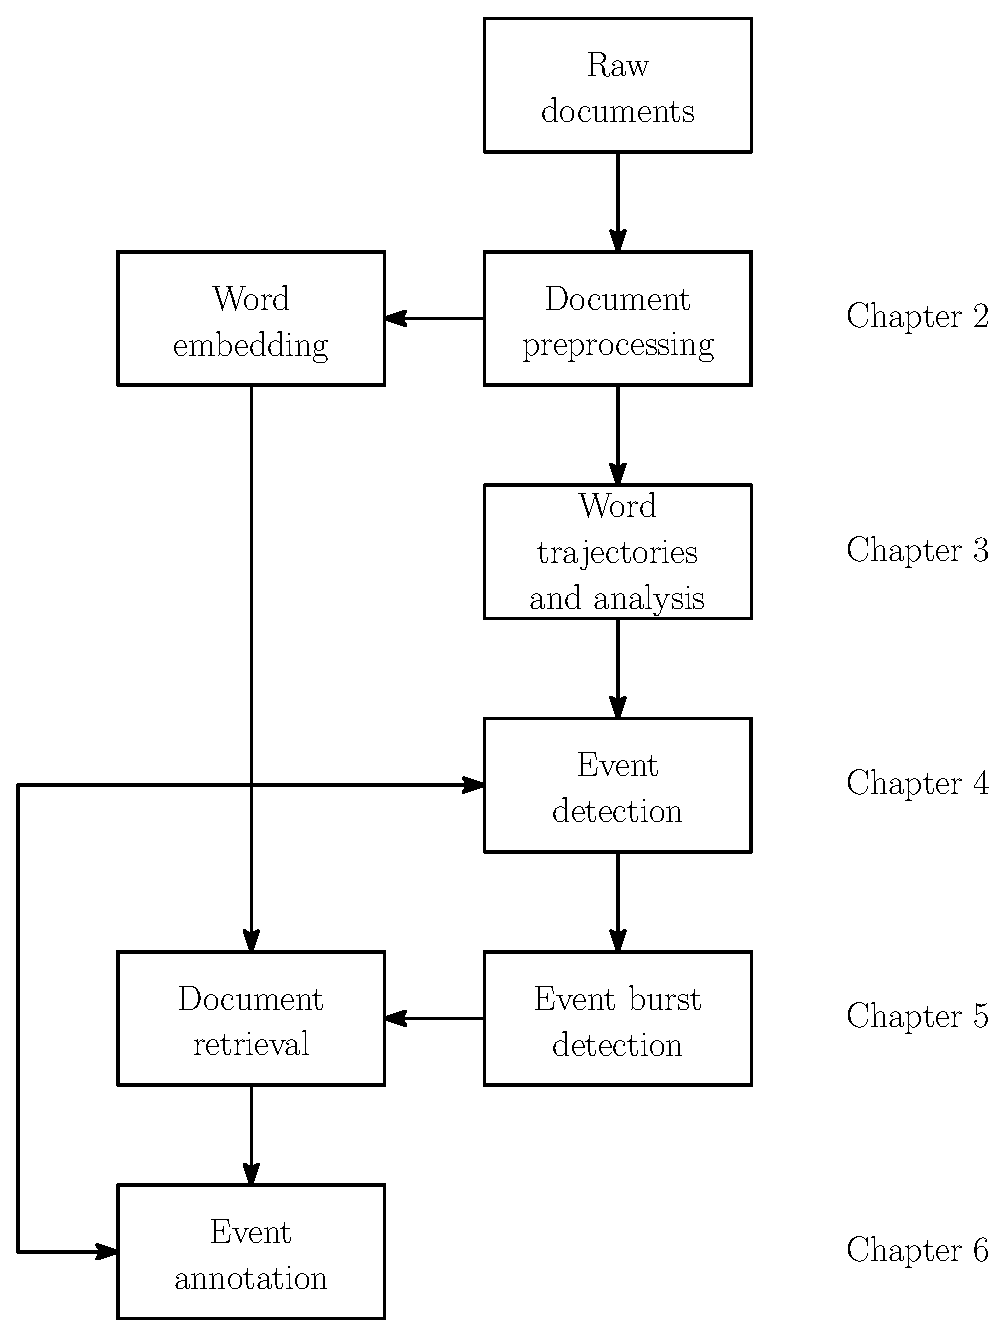
\includegraphics[height=0.6\paperheight]{diagram}
  \caption{Schematic representation of our method.}
  \label{fig:diagram}
\end{figure}

\chapter{Related work}
\label{chap:related-work}
A system encompassing event detection, subsequent document retrieval and automatic event annotation needs to tackle several issues. In particular, we need to select a suitable word embedding model to be used during the detection. Furthermore, we must decide on the detection method itself and also specify the process of relevant documents retrieval. Finally, we need to find a suitable method of annotating the detected events in a human-readable fashion.

All of these concerns have been addressed in literature. Below, we provide a basic overview of the related work which was helpful for our approach.


\section{Word embedding}
Recently, a number of neural network models for vector space word embedding have been proposed. Perhaps the best known model is Word2Vec \citep{word2vec} by Tomáš Mikolov. Additional methods include Stanford GloVe \citep{glove}, WordRank \citep{wordrank} and FastText \citep{fasttext}.

In this thesis, we use the Word2Vec model. The learned word vectors have useful semantical properties \citep{distributed-representations, linguistic-regularities}, an efficient implementation exists \citep{gensim}, and it is a well documented and accepted method.

The Word2Vec model has additionally been modified to support embedding whole documents \citep{doc2vec}.

\section{Event detection} \label{sec:related-event-detection}
Although our method is evaluated on a news collection, the documents do not necessarily have to come from a formal news source. A lot of work has also been published in event detection by analyzing tweets, an overview can be found in \cite{twitter-survey}, other examples being \cite{ifrim} and \cite{brigadir}. \cite{twitter-survey} also distinguish between \textit{retrospective} and \textit{online} event detection. The former analyzes a given collection of documents to discover past events, the latter (also known as \textit{First Story Detection}) tries to classify continuously incoming texts into ``old'' documents concerning events already known, and ``new'' documents concerning events not yet seen.

Further distinction can be made based on event representation. Some methods directly compare documents by their content and temporal similarity \citep{document-bursty-representation}, outputting an event as a set of documents. Others, such as \cite{parameter-free, event-detection, health-events} and our method included, represent the events by clusters of semantically and temporarily related keywords.

Additional work has also been done in event detection through topic modeling \citep{chaney, keane}. Topic modeling will be briefly addressed in the next section.

\section{Document retrieval}
Retrieving relevant documents from a large corpus based on a user-given query is the main concern of Information Retrieval \citep{information-retrieval-2, information-retrieval}. A number of methods comparing similarity of document representation through vectors has been created. These methods range from a simple, yet precise binary weighting \citep{luhn, salton, information-retrieval}, to those utilizing term weighting to diminish common words \citep{tfidf} and approaches that attempt to discover a latent structure behind the documents, such as Latent Semantic Indexing \citep{lsi}.

Further work has been done in topic modeling, where the focus is to discover abstract topics behind the documents. Latent Semantic Indexing belongs to topic modeling as well. More complex methods, such as Latent Dirichlet Allocation \citep{lda} employ a generative probabilistic model to discover the topical structure. Document can then be compared in terms of their topical similarity.

Recently, a new similarity measure utilizing the Word2Vec model, an extension of \cite{emd}, called Word Mover's Distance \citep{wmd} was introduced. This is a measure we are going to use and discuss in \autoref{chap:document-retrieval} in more detail.

\section{Event annotation}
For annotating the detected events, we consulted \cite{summarization-survey-1} and \cite{summarization-survey-2}. We aim to obtain a short summary for each event using the documents retrieved as relevant. The task of document summarization can be divided into \textit{abstractive}, where the task is to generate new sentences or words not seen in the documents, and \textit{extractive}, where the task is to extract parts of the document into a summary.

An example of the abstractive approach applied on news events is \cite{heady}, extractive approach is addressed by e.g. \cite{sum-multi, multi-summarization-1, multi-summarization-2}. The abstractive methods are much more complex and still an active area of research, as it is necessary to generate sentences with a logical structure. We decided to employ the extractive approach, as the methods are generally better documented, simpler and more mature.

The method introduced by \cite{multi-summarization-1, multi-summarization-2} supports multi-document summarization, which is suitable for our task, as we have multiple documents relevant to each event. Additionally, \cite{mogren-1} examined various ways of how this approach could be improved by word embeddings. Their work led to a system presented in \cite{mogren-2} which aggregates multiple similarity measures to perform summarization. We decided to adapt this system for our task.

\chapter{Document stream and preprocessing}
\label{chap:data-preprocessing}
The collection we work with comes directly from webscraping without any special structure. The documents consist only of headlines, bodies and publication days. Furthermore, there are some noisy patterns such as residual HTML entities, typos, words cut in the middle, etc. To make the most of the following methods, we preprocess the documents to remove as many of these errors as possible, and also to gain some additional information about the text.

We will first employ some NLP methods to gain insight into the data. Then, we will train a model to obtain word embeddings.

Since most machine learning methods rely on the data being represented numerically, usually in a vector space, it is necessary to obtain such representation from the basic words we work with. Preferably, these vectors should retain as much information as possible. There are many ways to do so --- a simple TFIDF representation \cite{information-retrieval} which represents the words by weighted counts of their appearance in the document collection. More complicated methods, such as Latent Semantic Indexing \cite{lsi} attempt to discover latent structure within words to also reveal topical relations between them. This idea is further pursued by probabilistic topical models, such as Latent Dirichlet Allocation \cite{lda}.

In this thesis, we use the \textit{word2vec} model introduced by Tomáš Mikolov \cite{distributed-representations, linguistic-regularities, word2vec}, which uses a shallow neural network to project the words from some vocabulary into a vector space. Vectors in this space have interesting semantical properties, such as vector arithmetics preserving semantic relations, or semantically related words forming clusters.

Later on, we will need to measure word similarity. This will come up several times in the process of event detection --- in the event detection itself, later when querying the document collection to obtain documents related to the detected events, and finally to compute human-readable summaries. The word2vec models is fit for all of these uses, as opposed to the other mentioned approaches, some of which are designed only to measure document similarity, or, on the other hand, do not support document similarity queries very well.


\section{Document collection}
The input to the algorithm is a collection of $\doccount$ news documents containing full text articles along with their publication days, headlines and, possibly, additional metadata. We assume no preprocessing was done prior to running the algorithm.

If we denote $t_{i}$ as the publication day of a document $d_{i}$, the collection can be understood as a stream $\left\{ (d_{1}, t_{1}), (d_{2}, t_{2}), \dots, (d_{\doccount}, t_{\doccount}) \right\}$ with $t_{i} \leq t_{j}$ for $i < j$. Furthermore, we define $\streamlen$ to be the length of the stream (in days), and we normalize the document publication days to be relative to the document stream start; that is $t_{1} = 1$ and $t_{\doccount} = \streamlen$.


\section{Dataset}
{\color{red} TODO: Describe the dataset.}


\section{Preprocessing}
Some of the documents contain residual HTML entities from errors during web scraping, which we filter out using a manually constructed stopwords list.

We used the MorphoDiTa tagger \cite{morphodita} to perform tokenization, lemmatization and parts-of-speech tagging. Our whole analysis will be run on these lemmatized texts, and we will revert to the full forms only at the end when summarizing the events in a human-readable way.

{\color{red} TODO: Mikolov's phrase detection model?}


\section{Word embeddings} \label{word-embeddings}
Here, we will train the mentioned word2vec model. Although the training is time-consuming, the word vectors can be pre-trained on a large document collection and then reused in following runs, even on different documents.

For the training, we only discard punctuation marks and word denoted as unknown parts of speech my the tagger. Such unknown words are mostly typos or foreign language terms not important for our analysis. We do not remove any additional stopwords or parts of speech, as this would break word order, which is, to some extent, used by the word2vec model.

The thesis was implemented using the Gensim \cite{gensim} package. The project contains memory efficient, easy to use Python implementations of various topic modeling algorithms, word2vec included. In addition, we used the SciPy toolkit \cite{scipy} and Scikit-Learn \cite{scikit-learn} for various machine learning-related computations.

{\color{red} TODO: Describe the settings used in the algorithm (vector space dimensionality, avg/concat, etc.)}

\chapter{Word-level analysis}
\label{chap:word-analysis}
This is the first phase of the event detection algorithm, focused on obtaining a set of candidate word features for event representation. We do not yet perform the actual event detection, which will be addressed in the next chapter, but merely extract a subset of words carrying enough information to be considered representative.

Here we work with the assumption that an event can be detected by observing the frequencies of individual words over time and grouping together those words which appear in similar documents during similar time periods \cite{event-detection, parameter-free}. This corresponds to an event being often mentioned in the text stream, be it a formal news stream or a stream of social network comments, around the period when it actually occurred. Of course, not all words are representative of an event, so we will have to impose a criterion of a ``word eventness''. Furthermore, there are some words appearing periodically during the duration of the text stream, such as words related to sport matches or weather forecasts reported every week. While they may be of interest, we will aim to distinguish them from words appearing only once during the observed period.

{\color{red} TODO: Pretty graphs of aperiodic vs. periodic trajectory}

At first, we will construct a trajectory of each word --- a measure of word frequency over time. We will then apply signal processing techniques to determine both eventness and periodicity of each word, and categorize the words accordingly into eventful-periodic and eventful-aperiodic, discarding the rest.

These trajectories will then be examined for so called ``bursts'' in frequency, where a word would suddenly appear in a large number of documents. Should a higher number of words appear in similar documents with overlapping bursts, it may be an indicator that an event worthy of attention occurred.

One thing to note is that the frequency of a word is, by itself, not a good indicator of a word importance.
Stopwords appearing in most documents, such as conjunctions, prepositions, etc. do not carry any information and should be ignored. Therefore, we will utilize the parts of speech tagging performed earlier and limit our analysis to Nouns, Verbs, Adjectives and Adverbs only.

{\color{red} TODO: Pretty graphs of eventful word vs. stopword trajectory}

This chapter focuses entirely on word analysis while ignoring the documents. Once we have assembled the words into events, we will return to document representation. The core of this algorithm is taken from \cite{event-detection}.


\section{Binary bag of words model}
To construct the word trajectories, we first need to know which words appear in which documents, as we are interested in the document frequency of each word. We will create a binary bag of words model, which is represented by a binary matrix denoting the incidence of documents and words. This model completely ignores word order, which is not necessary for this analysis, and was considered previously in word embeddings.

We define a term-document matrix $\bowmat \in \left\{ 0, 1 \right\}^{\doccount \times \featcount}$, where $\doccount$ is the number of documents and $\featcount$ is the total vocabulary size. The document collection can then be interpreted as a set of $\doccount$ observations, each consisting of $\featcount$ binary features. The matrix $\bowmat$ is defined as

\begin{equation} \label{eq:bow-matrix}
	\bowmat_{ij} \coloneqq
	\begin{cases}
		1, & \text{document}~i~\text{contains the word}~j \text{;} \\
		0, & \text{otherwise.}
	\end{cases}
\end{equation}

{\color{red} TODO: Figure out the min\_freq and max\_freq of words to keep.}

To further limit the feature space, we discard words appearing in less than 30 documents or in more than 90\% of the documents. The idea behind this is that the words appearing only in few documents cannot possibly represent relevant events, and are mostly anomalies or typos. On the other hand, words appearing in most of the documents are likely stopwords, and do not carry much information. This helps to prune the feature space and makes $\bowmat$ reasonably sized.


\section{Computing feature trajectories}
The time trajectory of a word feature $f$ is a vector $\vect{\traj}_{f} = \left[ \traj_{f}(1), \traj_{f}(2), \dots, \traj_{f}(\streamlen) \right]$ with each element $\traj_{f}(t)$ being the relative frequency of $f$ at time $t$. This frequency is defined using the DFIDF score:

\begin{equation}
	\traj_{f}(t) \coloneqq \underbrace{\frac{\text{\df}_{f}(t)}{\text{\doccount}(t)}}_{\text{DF}} \cdot \underbrace{\log{\frac{\doccount}{\text{\df}_{f}}}}_{\text{IDF}},
\end{equation}

where $\text{\df}_{f}(t)$ is the number of documents published on day $t$ containing the feature $f$ (time-local document frequency), $\text{\doccount}(t)$ is the number of documents published on day $t$ and $\text{\df}_{f}$ is the number of documents containing the feature $f$ (global document frequency).

These feature trajectories are stored in a matrix $\trajmat \in \R^{\featcount \times \streamlen}$, with $\vect{\traj}_f$ being the $f$-th row of $\trajmat$. Here we take advantage of the normalization of the publication days, since they can now be used as column indices of $\trajmat$.

To make the computation efficient, we vectorize most of the operations. Along with the matrix $\bowmat$ defined in \ref{eq:bow-matrix}, we define a matrix $\dtdmat \in \left\{ 0, 1 \right\}^{\doccount \times \streamlen}$ mapping the documents to their publication days:

\begin{equation}
	\dtdmat_{ij} \coloneqq
	\begin{cases}
		1, & \text{document}~i~\text{was published on day}~j \text{;} \\
		0, & \text{otherwise}.
	\end{cases}
\end{equation}

Next, we sum the rows of $\bowmat$ together to obtain $\vect{\df} = \left[ \text{\df}_{1}, \text{\df}_{2}, \dots, \text{\df}_{\featcount} \right]$, and similarly the rows of $\dtdmat$ to obtain $\vect{\doccount}_{t} = \left[ \text{\doccount}(1), \text{\doccount}(2), \dots, \text{\doccount}(\streamlen) \right]$.

Using these matrices and vectors, we can compute $\trajmat$ as follows:

\begin{equation}
	\trajmat \coloneqq
		\underbrace{\text{diag} \left( \log{\frac{\doccount}{\vect{\df}}} \right)}_{\text{IDF}}
		\cdot
		\underbrace{\bowmat^{\T}
		\cdot \dtdmat
		\cdot \text{diag} \left( \frac{1}{\vect{\doccount}_{t}} \right)}_{\text{DF}}
\end{equation}

Now, every word feature $f$ is represented by two vectors --- $\vect{\traj}_{f}$ being its time trajectory, and $\embed_{f}$ being its word embedding. We obtained temporal and semantic representation of the words, both of which will be utilized for event detection in the next chapter.


\section{Spectral analysis}
Having constructed the word trajectories, we still need to decide which words are eventful enough, and also categorize them into periodic and aperiodic. We interpret the trajectories as time signals, which allows us to employ spectral analysis techniques to discover periodicities and estimate signal power. The words with high enough signal power will then be deemed as eventful.

We apply the discrete Fourier transform to each trajectory to represents the time series as a linear combination of $\streamlen$ complex sinusoids. We obtain $\mathcal{F} \vect{\traj}_{f} = \left[ X_{1}, X_{2}, \dots, X_{\streamlen}\right ]$ such that

\begin{equation*}
	X_{k} = \sum_{t = 1}^{\streamlen}{\traj_{f}(t) \exp(- \frac{2 \pi \mi}{\streamlen} (k - 1) t}), ~ k = 1, 2, \dots, \streamlen.
\end{equation*}

Having moved from the time domain to the frequency domain, we can now analyze the signal power and dominant periodicity of each word. They will be obtained from the power spectrum of the transformed trajectories, which is estimated using the periodogram estimator

\begin{equation*}
	\vect{P} = \left[ \|X_{1}\|^{2}, \|X_{2}\|^{2}, \dots, \|X_{\ceil{\streamlen / 2}}\|^{2} \right].
\end{equation*}

To measure the overall signal power, we define the dominant power spectrum of the word feature $f$ as the value of the highest peak in the power spectrum, that is

\begin{equation}
	\text{DPS}_{f} \coloneqq \max\limits_{k \leq \ceil{\streamlen / 2}}{\|X_{k}\|^{2}}.
\end{equation}

The dominant period is then defined as the inverse of the frequency corresponding to the highest peak:

\begin{equation}
	\text{DP}_{f} \coloneqq \frac{\streamlen}{\argmax\limits_{k \leq \ceil{\streamlen / 2}}{\|X_{k}\|^{2}}},
\end{equation}

{\color{red} TODO: Plot graphs of periodic and aperiodic word showing both time trajectory and its Fourier transform}

When applied to rows of the matrix $\trajmat$, this method yields two vectors $\vect{DPS},\ \vect{DP} \in \R^{\featcount}$, containing the dominant power spectra and dominant periods, respectively.


\section{Feature categorization}
Based on the dominant power spectra and dominant periods, we divide the word features into \underline{E}ventful-\underline{A}periodic and \underline{E}ventful-\underline{P}eriodic categories \footnote{\cite{event-detection} actually define \textit{five} such categories; however, our method uses only the two sets of the most powerful features.}:

\begin{equation}
\begin{split}
	\text{EA} \coloneqq \left\{ f \mid \text{DPS}_{f} > \textit{dps-bound},\ \text{DP}_{f} > \ceil{\streamlen / 2} \right\}, \\
	\text{EP} \coloneqq \left\{ f \mid \text{DPS}_{f} > \textit{dps-bound},\ \text{DP}_{f} \leq \ceil{\streamlen / 2} \right\}.
\end{split}
\end{equation}

{\color{red}TODO: Define dps-bound!}

\chapter{Event detection algorithms}
\label{chap:event-detection}
In this chapter, we describe the actual event detection algorithm. First, we describe the original method used by \cite{event-detection}. Then, we will make a change to incorporate semantic similarity through the word embeddings obtained in \autoref{chap:data-preprocessing}. Finally, we introduce an alternative algorithm that depends on word clustering using a custom distance function.

The original algorithm creates events as sets of related keywords by greedily minimizing a cost function combining temporal and semantical distance between words. However, the paper used only a simple notion of semantical distance, namely the document overlap between words. This demands that there exists at least one document containing all the words used to represent an event. This is a strong requirement, since the documents may use different vocabularies while conveying similar information.  As a result, the events are split into multiple keyword sets, leading to redundancy.

In an attempt to solve this problem, we modify the cost function, replacing the document overlap by Word2Vec-based similarity. This does not require the words to appear in exactly the same documents, only that they have similar semantics. We refer to this method as \textit{greedy approach}.

Realizing that the task of constructing keyword sets resembles the task of word clustering, we propose an alternative algorithm. Here, we apply a clustering algorithm to the words, using a modification of the cost function as a distance measure. This is a method referred to as \textit{cluster-based approach}.

First, we briefly describe the original method for referrence. This will make it clear which parts of the function we modify. It will also allow us to make reference to the original method in \autoref{chap:evaluation}, where we compare all three algorithms.

\section{Original method}
As stated in the introduction, the original method performs greedy minimization of a cost function defined over sets of words. The cost function consists of trajectory distance measuring the word distance in temporal domain, and document overlap, standing for distance in the semantic domain. We will first describe these two components and then combine them into the cost function.

\subsection{Trajectory distance}
Before measuring the trajectory distance, the trajectories are smoothened by fitting a probability density function to them. We adapt a similar technique in \autoref{chap:document-retrieval} where it is described in more detail. Our event detection modifications do not use it though, and we refer the reader to the original paper for more details.

After normalization to unit sum, the (smoothened) trajectory $\vect{\traj}_{w}$ of a word $w$ can be interpreted as a probability distribution over the stream days. The element $\traj_{w}(i)$ then denotes the probability that $w$ appears on day $i$. This interpretation allows to compare the trajectories using information-theoretic techniques, notably the information divergence.

In the original paper, the authors first defined the distance between trajectories of two words $v$ and $w$ as $\trajdist{\vect{\traj}_{v}}{\vect{\traj}_{w}} = \max \left\{ \kl{\vect{\traj}_{v}}{\vect{\traj}_{w}}, \kl{\vect{\traj}_{w}}{\vect{\traj}_{v}} \right\}$, symmetrizing the Kullback-Leibler divergence KL.

Then, the distance is generalized to a whole set of words $\featset$ as

\begin{equation}
	\text{Dist}( \featset ) = \max_{v, w \in \featset} \trajdist{\vect{\traj}_{v}}{\vect{\traj}_{w}}.
\end{equation}

\subsection{Document overlap}
The document overlap is again first defined for a pair of words $v$ and $w$ as $\text{DO}\left( v, w \right) = \frac{| \featset_{v} \cap \featset{w} |}{\min \left\{ | \featset_{v} |, | \featset_{w} | \right\}}$, where $\featset_{i}$ is the set of all documents containing the word $i$. The higher the document overlap, the more documents do the two words have in common, which them more likely to be correlated.

The overlap is again generalized to a set of words $\featset$ as

\begin{equation}
	\text{DO}( \featset ) = \min_{v, w \in \featset} \text{DO}( v, w ).
\end{equation}

\subsection{Cost function}
The cost function is a combination of the trajectory distance and document overlap of a set of words. It is defined as

\begin{equation}
	\text{C}( \featset ) = \frac{\text{Dist}( \featset )}{\text{DO}( \featset ) \cdot \sum_{w \in \featset} \text{DPS}_{w}}.
\end{equation}

Since the algorithm will attempt to minimize it, the intuitive result will be a set of words with with low trajectory distance and high document overlap. The algorithm will also prefer words of higher importance due to the last term of the denominator, counting in the power spectra.

\newpage

\subsection{Event detection algorithm}
The algorithm, called \textit{unsupervised greedy event detection algorithm} in the original paper, is defined as follows.

\begin{algorithm}[H]
\begin{algorithmic}[1]
\caption{Unsupervised greedy event detection}
\label{alg:greedy-event-detection}
\Input $\text{Word set} ~ \featset$

\State $\text{Sort the words in descending DPS order: } DPS_{w_{1}} \geq \dots \geq DPS_{w_{\left\vert \featset \right\vert}}$

\State $k = 0$

\ForEach{$w \in \featset$}
	\State $k = k + 1$	
	\State $e_{k} = \{ w \}$
	\State $cost_{e_{k}} = \frac{1}{DPS_{w}}$
	\State $\featset = \featset \setminus w$
	
	\While{$\featset \neq \emptyset$}
		\State $m = \argmin\limits_{m}{\text{C}( e_{k} \cup w_{m} )}$

		\If{$\text{C}( e_{k} \cup w_{m} ) < cost_{e_{k}}$}
			\State $cost_{e_{k}} = \text{C}( e_{k} \cup w_{m} )$
			\State $e_{k} = e_{k} \cup w_{m}$
			\State $\featset = \featset \setminus w_{m}$
		\Else
			\Break
		\EndIf
	\EndWhile
\EndFor

\Output $\text{Events} ~ \{ e_{1}, \dots, e_{k} \}$
\end{algorithmic}
\end{algorithm}


\begin{figure}[H]
  \centering
  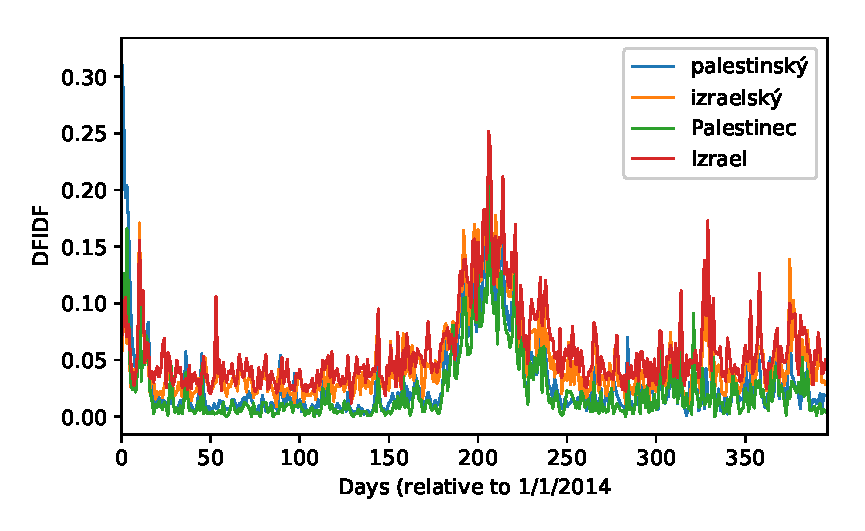
\includegraphics{original_event}  % original event
  \caption{Example of an event detected using the original method. The event consists of the words \textit{palestinian}, \textit{israeli}, \textit{Palestinian} and \textit{Israel}, respectively.}
  \label{fig:original-event}
\end{figure}


\section{Greedy approach}
Here, we describe the modifications done to the original method. We change the semantic similarity measure to take advantage of the Word2Vec model, and also redefine the trajectory distance accordingly, so it takes a similar form.

Both measures will be defined directly between a set of words $\featset$ and another word $w \notin \featset$.

\subsection{Trajectory distance}
We assume that the trajectories have been normalized to unit sum, as in the original method. The trajectory distance of $w$ to $\featset$ is again defined defined in terms of the Kullback-Leibler divergence as

\begin{equation}
	\trajdist{\featset}{w} = \kl{\vect{\bar{\traj}}_{\featset}}{\vect{\traj}_{w}},
\end{equation}

where $\vect{\bar{\traj}}_{\featset}$ is the mean of all trajectories of $\featset$ and $\vect{\traj}_{w}$ is the trajectory of $w$. The advantage is that, unlike in the original method, the divergences do not need to be precomputed between all pairs of words. The distance between a set and another word can be computed directly during the detection process, saving computation time.


\subsection{Semantic similarity}
Some of the astounding results of the Word2Vec model arise from semantically similar words forming clusters \citep{linguistic-regularities} in terms of cosine similarity, which is a standard measure used in information retrieval \citep{information-retrieval, cosine-similarity}.

The semantic similarity of $\featset$ and $w$ is defined in terms of cosine similarity as

\begin{equation}
	\semsim{\featset}{w} = \frac{\inp[\big]{\bar{\embed}_{\featset}}{\embed_{w}}}{\| \bar{\embed}_{\featset} \| \cdot \| \embed_{w} \|},
\end{equation}

where $\bar{\embed}_{\featset}$ is the mean of all vector embeddings of $\featset$ and $\embed_{w}$ is the vector embedding of $w$. Here, the mean vector represents the central topic of words in $\featset$.


\subsection{Cost function}
The cost function is defined similarly as in the original method:

\begin{equation} \label{eq:cost-function}
	\cost{\featset}{w} = \frac{\trajdist{\featset}{w}}{\exp(\semsim{\featset}{w}) \cdot \sum_{g \in \featset \cup w}{\text{DPS}_{g}}},
\end{equation}

Since the cosine similarity is bounded in $[-1, 1]$, we exponentiate it so that it is always positive. Otherwise, the cost function would reach negative values for highly dissimilar words, which would minimize it more than for similar ones.

Having constructed the cost function, we use Algorithm \ref{alg:greedy-event-detection} to detect events once again.


\begin{figure}[H]
  \centering
  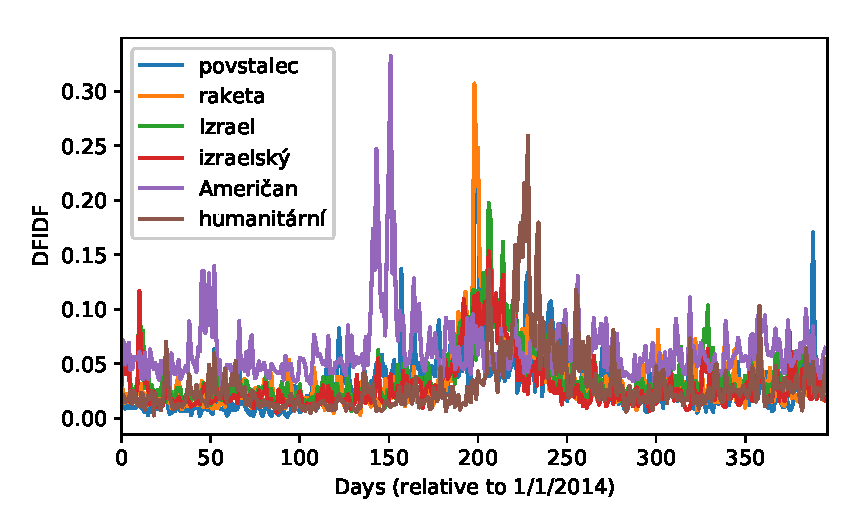
\includegraphics{greedy_event}  % greedy event
  \caption{Example of an event detected using the greedy method. The event consists of the words \textit{to shoot}, \textit{missile}, \textit{Israel} and \textit{israeli}, and is related to the same real event as \autoref{fig:original-event}.}
  \label{fig:greedy-event}
\end{figure}


\section{Cluster-based approach}
The final method interprets the task as literal clustering of words, using a custom distance function. The distance function will actually be a modification of the cost function yet again, though some means have to be taken to make it usable in this context. First, we need to consider a proper clustering algorithm.

The obvious requirement for the clustering algorithm is that it must not require an a priori knowledge of the desired number of clusters. Another requirement is that the algorithm must accept a custom distance measure.

We considered three candidate algorithms: Affinity propagation \citep{affinity-propagation}, DBSCAN \citep{dbscan} and its modification, HDBSCAN \citep{hdbscan}.

During our experimentation, Affinity propagation performed poorly, its clusters being often seemingly random and of low quality. The quality of HDBSCAN clusters was considerably better, though the algorithm took longer to converge as the number of eventful words grew. It also required to tune multiple parameters, which was difficult to do without any annotated data. We decided to use the DBSCAN algorithm, which outperformed Affinity propagation as well, and does not require to tune as many parameters as HDBSCAN.

In addition to the previously stated requirements, DBSCAN is also capable of filtering out noisy samples, not fit for any of the clusters. This property will prove advantageous for our task, as will become clear during the evaluation in \autoref{chap:evaluation}.


\subsection{Noise filtering}
Before we apply clustering, we will filter out the noisy parts from the word trajectories. Most words are on some level reported all the time, though only a fraction of these reportings corresponds to notable events. Unlike the greedy optimization described previously, clustering is prone to such noise, and would yield clusters of poor quality, often with trajectories being put together only due to their noisy parts being similar. With DBSCAN capable of filtering out noisy samples, quality words with some noise in their trajectories would be discarded.

We want to keep only those trajectory parts exceeding a certain frequency level, distinguishing notable bursts from the general noise. We do this by computing a cutoff value for each event trajectory and discarding the sectors falling under this cutoff. This procedure is adopted from \cite{online-search-queries}. The algorithm is based on computing a moving average along the trajectory, and works as follows:

\begin{algorithm}[H]
\begin{algorithmic}[1]
\caption{Burst filtering}
\label{alg:burst-filtering}
\Input $\text{window-length} \ l,\ \text{word trajectory} \ \vect{\traj_{w}}$

\State $\vect{MA}_{l} = \text{Moving Average of length} ~ l ~ \text{for} ~ \vect{\traj}_{w} = \left[ \traj_{w}(1), \traj_{w}(2), \dots, \traj_{w}(\streamlen) \right]$

\State $\mathit{cutoff} = \text{mean} \left( \vect{MA}_{l} \right) + \text{std} \left( \vect{MA}_{l} \right)$

\State $\vect{bursts}_{w} = \left[ \traj_{w}(t) \mid \traj_{w	}(t) > \mathit{cutoff} \right]$

\Output $\vect{bursts}_{w}$
\end{algorithmic}
\end{algorithm}


\subsection{Distance function}
We now define the distance function used by DBSCAN. It conveys similar information as the cost function in the previous two algorithms. We still need to measure the trajectory distance as well as semantic similarity between two words.

For a measure of trajectory distance, we replace the Kullback-Leibler divergence by the Jensen-Shannon divergence JSD, which is symmetric in its arguments. This is a necessary property of the distance function.

Instead of semantic \textit{similarity}, we measure semantic \textit{distance} as the Euclidean distance between two word vector embeddings. The reason is that Euclidean distance is unbounded, which makes it possible for the samples to be spread farther apart. Since DBSCAN is a density-based clustering algorithm, having high density areas consisting of words with low trajectory distance and similar cosine similarities would cause them to appear in the same cluster. This would cluster the words only in terms of their trajectories, not semantics.

The distance between two words $v$ and $w$ with trajectories $\vect{\traj}_{v},\ \vect{\traj}_{w}$ and embeddings $\embed_{v},\ \embed_{w}$ is now defined as

\begin{equation}
	\distfunc{v}{w} = \jsd{\vect{\traj}_{v}}{\vect{\traj}_{w}} \cdot \| \embed_{v} - \embed_{w}\|_{2},
\end{equation}

with $\jsd{\vect{p}}{\vect{q}} = \frac{1}{2} \left( \kl{\vect{p}}{\vect{m}} + \kl{\vect{q}}{\vect{m}} \right) ,\ \vect{m} = \frac{1}{2} \left( \vect{p} + \vect{q} \right)$.


\subsection{Event detection}
The input and output of the event detection algorithm remains the same as in Algorithm \ref{alg:greedy-event-detection}, only the internals are different. This makes it easy to swap the two algorithms for comparison.

\begin{algorithm}[H]
\begin{algorithmic}[1]
\caption{Cluster-based event detection}
\Input $\text{Word set} ~ \featset$

\State Precompute a distance matrix $\distmat \in \R^{\left\vert \featset \right\vert \times \left\vert \featset \right\vert}$ with $\distmat_{ij} = \distfunc{w_{i}}{w_{j}}$

\State Apply HDBSCAN to $\distmat$, obtaining $k$ clusters and the noisy cluster

\ForEach{$(w, cluster) \in \text{HDBSCAN.clusters}$}
	\If{$cluster \neq noise$}
		\State $e_{cluster} = e_{cluster} \cup w$
	\EndIf
\EndFor

\Output $\text{Events} ~ \{ e_{1}, e_{2}, \dots, e_{k} \}$
\end{algorithmic}
\end{algorithm}


\begin{figure}[H]
  \centering
  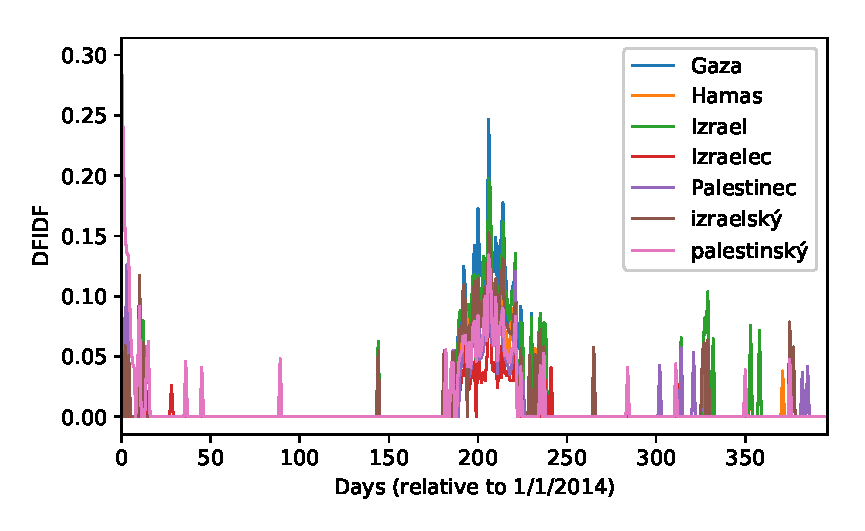
\includegraphics{cluster_event}  % cluster event
  \caption{Example of an event detected using the cluster-based method. The event is related to the same real event as \autoref{fig:original-event} and \autoref{fig:greedy-event}. Note that the trajectories are clear of noise due to application of Algorithm \ref{alg:burst-filtering}}
  \label{fig:cluster-event}
\end{figure}


\chapter{Document retrieval}
\label{chap:document-retrieval}
As our goal is to obtain a human-readable event description, we will need to move on from keyword representation to document representation, i.e. for each event, retrieve a number of documents concerning the particular event.

We can use each event's temporal and semantic information to query the document collection. The former is trivial -- simply select the documents published within an event's bursty period. The latter will prove more complicated, and we will need to employ some more information retrieval techniques to obtain semantically similar documents.

As of now, an event $e$ is described by a set of its keywords, $\kw{e}$. The goal is to convert this keyword representation to a document representation, $\doc{e}$ of documents related to $e$.

\section{Event burst detection}
First, we need to detect the period where the particular event occurred, so that we can retrieve the documents published around that time. We do this in four steps:

\begin{enumerate}
	\item Construct the event trajectory
	\item Clean the trajectory
	\item Fit a probability density function
	\item Take the region(s) with the highest density as the bursty period(s)
\end{enumerate}


\subsection{Event trajectory construction}

We will first need to construct an \textit{event trajectory} out of its \textit{keyword trajectories}. We do this by computing a weighted average of the event's keyword trajectories, with weights being the keyword DPS. This ensures that less important words with slightly different time characteristic will not shift the trajectory away from the actual burst.

\begin{equation}
	\vect{\traj_{e}} \coloneqq \frac{1}{\sum_{k \in \kw{e}}{\text{DPS}_{k}}} \sum_{k \in \kw{e}}{\text{DPS}_{k} \cdot \vect{\traj}_{k}}
\end{equation}


\subsection{Trajectory filtering}

Now, a typical event (shown in {\color{red} TODO: Put a pretty picture here}) will usually have some number of dominant bursts corresponding to the period(s) when the event actually occurred. Additionally, there will be some milder, noisy bursts due to the keywords appearing elsewhere, independently of that particular event. We are only interested in the main burst(s), and so we will need to filter out the noise.

We do this by computing a cutoff value for each event trajectory and discarding the sectors falling under this threshold. This procedure is adopted from \cite{online-search-queries}. The algorithm is as follows:

\begin{algorithm}[H]
\begin{algorithmic}[1]
\caption{Burst filtering}
\Input $\text{window-length} \ w,\ \text{event trajectory} \ \vect{\traj_{e}}$

\State $\vect{MA}_{w} = \text{Moving Average of length} ~ w ~ \text{for} ~ \vect{\traj}_{e} = \left[ \traj_{e}(1), \traj_{e}(2), \dots, \traj_{e}(\streamlen) \right]$

\State $\mathit{cutoff} = \text{mean} \left( \vect{MA}_{w} \right) + \text{std} \left( \vect{MA}_{w} \right)$

\State $\vect{bursts}_{e} = \left[ \traj_{e}(t) \mid \traj_{e}(t) > \mathit{cutoff} \right]$

\Output $\vect{bursts}_{e}$
\end{algorithmic}
\end{algorithm}

{\color{red} TODO: In the paper, they use $\vect{MA}(t)_{w} > \mathit{cutoff}$, try that. Also, why did I miss that? :(}

We further normalize the filtered trajectories to have unit sums, so they can be interpreted as probability distribution over the stream. An element $\traj_{e}(i)$ of the trajectory will denote a probability of that event occurring on day $i$. This allows us to fit a probability density function to them. \cite{event-detection} adapted a similar approach, though only for feature trajectories rather than event trajectories.

\subsection{Density fitting}
We describe aperiodic and periodic events separately, as different probability distributions must be used in case of a single burst than in case of multiple bursts.

\begin{enumerate}

\item \textbf{Aperiodic features}

An aperiodic feature trajectory $\traj_{f}$ is modeled by a Gaussian distribution. We fit the Gaussian function

\begin{equation*}
	f(x) = \frac{1}{\sigma \sqrt{2 \pi}} \exp(-\frac{\left( x - \mu \right)^{2}}{2 \sigma^{2}})
\end{equation*}

to the trajectory $y_{f}$. The parameters $\mu$ and $\sigma$ are estimated using non-linear least squares method. Unlike \cite{event-detection} who use the EM algorithm, least squares proved to be less prone to outliers, yielding a shape more resembling the actual trajectory.

\item \textbf{Periodic features}

A periodic feature trajectory $\traj_{f}$ is modeled using a mixture of $K = \floor{\streamlen / \text{DP}_{f}}$ Cauchy distributions (as many mixture components as there are periods), as in \cite{health-events}:

\begin{equation*}
	f(x) = \sum_{k = 1}^{K}{\alpha_{k} \frac{1}{\pi} \left( \frac{\gamma_{k}}{\left( x - \mu_{k} \right)^{2} + \gamma_{k}^{2}} \right)}
\end{equation*}

The mixing parameters $\alpha_{k},\ \sum_{k = 1}^{K}{\alpha_{k}} = 1$, location parameters $\mu_{k}$ and scale parameters $\gamma_{k}$ are estimated using the EM algorithm.

The Cauchy distribution has a narrower peak and thicker tails than the Gaussian distribution, which models the periodic bursts more closely. The individual bursts of a periodic feature tend to be quite short, but even between two consecutive bursts, the frequency remains at a non-negligible level, which makes the Cauchy distribution a somewhat better choice.


\subsection{Burst detection}
The bursty period of an aperiodic event is now defined as $\interval{\mu - \sigma}{\mu + \sigma}$. For a periodic event, there are $K = \floor{\streamlen / \text{DP}_{f}}$ bursty periods, each defined as $\interval{\mu_{k} - \gamma_{k}}{\mu_{k} + \gamma_{k}}$.



\section{Document retrieval}
We only describe the process for aperiodic events. The method is similar for periodic events, except applied on each burst individually.

Intuitively, we need to select some number of documents best representing an event $e$ out of all documents published within the event's bursty period. The only measure of semantics for an event we have is the event's keyword set $\kw{e}$. If we interpret $\kw{e}$ as a keyword query for the document collection, we arrive at the classical task of information retrieval.

In the original method by \cite{event-detection}, the task was simple due to the cost function used. In the paper, the only measure of semantic related-ness used was the degree of document overlaps. That way, there was always at least one document in which all of the event's keywords appeared. This is not the case in our method, and we will need to measure the semantic similarity in a more sophisticated way.

There are a number of approaches we could take, such as project all documents and queries to a TFIDF space \cite{information-retrieval} and sort the documents by their cosine similarity to the query. This simple approach does not go beyond a simple keyword occurrence. We could enrich it using Latent Semantic Indexing \cite{lsi} to also take the document topics into account. This would however require us to ``train'' yet another model for this task only, which would be computationally and memory-intensive.

Instead, we decided to further utilize the trained Word2Vec model and use the recently introduced Word Mover's Distance \cite{wmd}.

The Word Mover's Distance (WMD) is a novel measure of document similarity based on Word2Vec embeddings of the document words. The similarity of two documents is measured as the minimum distance the word vectors of one document need to ``travel'' to reach the word vectors of the second document.

The WMD discards word order, which makes it suitable for our keyword queries. As the authors note, it achieves best results for short documents, in part due to the method being computationally expensive for larger pieces of text. Therefore, we apply the WMD on document headlines only.

Since the WMD is a measure of distance, we use the WMD similarity instead, defined as

\begin{equation}
	\wmdsim{d_{i}}{d_{j}} \coloneqq \frac{1}{1 + \wmd{d_{i}}{d_{j}}}
\end{equation}

\begin{algorithm}[H]
\begin{algorithmic}[1]
\caption{Document representation of an event}
\Input $\text{Event}\ e,\ \text{number of documents}\ n,\ \text{document stream}\ D$

\State $\mathit{burst\_docs} = \emptyset$

\ForEach{$\mathit{doc} \in D$}
	\If{$\mathit{doc.publication\_date} \in \mathit{e.burst}$}
		\State $\text{Compute}\ \wmdsim{\kw{e}}{\mathit{doc.headline}}$
		\State $\mathit{burst\_docs} = \mathit{burst\_docs} \cup \mathit{doc}$
	\EndIf
\EndFor

\State $\text{Sort}\ \mathit{burst\_docs}\ \text{by the computed}\ \text{Sim}_{\text{WMD}} \ \text{in descending order}$
\Output $\doc{e} = \text{first}\ n\ \text{elements of}\ \mathit{burst\_docs}$
\end{algorithmic}
\end{algorithm}

\end{enumerate}

\chapter{Event annotation}
\label{chap:event-annotation}
The final step of our method is to annotate the detected events in a human-readable way. We aim to generate short summaries so that the user does not have to process a large quantity of text, and can just skim through a few sentences to decide whether they are interested in that particular event. If so, then they can examine the event more closely and go through the actual documents, which we have retrieved in chapter \autoref{chap:document-retrieval}.

Although the keyword set discovered in \autoref{chap:event-detection} provides a concise representation of an event, it can lead to ambiguities or simply not reveal enough information. {\color{red} TODO: Add an example of an event not well recognizable by its keyword set.} The keywords should be considered an internal representation used in the detection process, not something presentable to the user.

A simple method is to annotate an event by the headline of the most relevant document in terms of Word Mover's Similarity. This may give insight of the general topic of the particular event, but it is unlikely that a whole event will be well characterized by a single document. For this reason, we also investigate a more complex method. Nevertheless, we will provide such headlines for comparison.

The second approach is to use multi-document summarization techniques to generate a short summary of an event's document set. More specifically, we attempt to extract some number of sentences from the document set which cover the general topic of the set without providing redundant information. As the documents come from different sources and describe the events from different perspectives, the result will not generally be a continuous paragraph, but more of a set of characteristic sentences. Still, a longer piece of text will likely provide a better insight into an event than a single headline.

We use the multi-document summarization system presented in \cite{multi-summarization-1, multi-summarization-2}, which we describe in more detail in the following paragraphs. This system was later improved by \cite{mogren-1}, who evaluated the usage of different word embedding techniques for sentence similarity measures. Their work led to the system presented in \cite{mogren-2} which aggregates several different similarity measures to obtain a better quality summary.


\section{Multi-document summarization}
In \cite{multi-summarization-1}, the authors formulate the task of multi-document summarization as a constrained combinatorial optimization problem, where the goal is to retrieve a subset of sentences maximizing a monotone submodular function $\quality{\cdot}$ measuring the summary quality.

A submodular function $\quality{\cdot}$ on a set of sentences $V$ satisfies the property of \textit{diminishing returns}; that is, for $A \subseteq B \subseteq V \setminus \{ v \},\ \quality{A \cup \{ v \}} - \quality{A} \geq \quality{B \cup \{ v \}} - \quality{B},\ v \in V$. This has intuitive explanation for text summarization, namely that adding a sentence $v$ to a longer summary does not improve the summary as much as adding it to a smaller one. The reason is that the information carried by $v$ is more likely present in the longer summary already.

Even though solving the task exactly is NP-hard, a greedy algorithm is guaranteed to find a solution inly a constant factor off the optimum, as discussed by the authors.

The summary quality is measured in terms of how representative it is to the whole set (coverage) and how dissimilar the sentences are to each other (diversity). The constraints limit the summary to a reasonable length by bounding either the number of sentences or the number of words.

In \cite{multi-summarization-1}, basic submodular functions to be used in multi-document summarization are described. In \cite{multi-summarization-2}, these functions are further developed to better capture the semantic properties.

Mathematically, the task is formulated as

\begin{equation}
\begin{alignedat}{-1}
\max_{S \subseteq V} & \quad \quality{S} = \coverage{S} + \lambda \diversity{S} \\
\text{s. t.} & \quad \sum_{i \in S}{\sentcost_{i}} \leq \budget,
\end{alignedat}
\end{equation}

where $V$ is the set of all sentences from the document set being summarized, $\sentcost_{i}$ is the cost of sentence $i$ (either 1 when limiting the number of sentences or the number of words in the sentence) and $\budget$ is the total budget.

A feasible set $S$ maximizing $\quality{\cdot}$ will provide a reasonable number of sentences well capturing the overall topic of the whole document set, no two of which being redundant. What remains is to define the coverage function $\coverage{\cdot}$ and diversity function $\diversity{\cdot}$, whose influence can be controlled by the parameter $\lambda \geq 0$. Additionally, the functions must be defined in a way that the conditions from \cite{multi-summarization-1} are not broken, so that a greedy algorithm can still be used.


\section{Coverage function}

In \cite{multi-summarization-2}, the coverage function $\coverage{\cdot}$ is defined in terms of pairwise sentence similarity $\semsim{\cdot}{\cdot}$ as

\begin{equation}
\coverage{S} = \sum_{i \in V}{\min{\Big\{ \sum_{j \in S}{\semsim{i}{j}}, \alpha \sum_{k \in V}{\semsim{i}{k}} \Big\} }}.
\end{equation}

The first argument measures the similarity between the sentence $i$ and the summary $S$, while the second argument measures the similarity between the sentence $i$ and the rest of the sentences $V$. The number $\alpha \in [0,1]$ is a threshold coefficient.

The authors further prove that if $\semsim{i}{j} \in [0,1]\ \forall i, j \in V$, the whole function remains submodular. {\color{red} TODO: Where was that?}

Originally, only a simple cosine similarity between TFIDF sentence vectors \cite{information-retrieval} was used in $\semsim{\cdot}{\cdot}$. Kågebäck et al. examined various methods of word embeddings in \cite{mogren-1} to obtain a finer measure of similarity. This alone outperformed the original method, and in \cite{mogren-2}, a more complex system aggregating multiple similarity measures was built. We use this method with several different similarity measures fit for the event detection task.

The sentence similarity $\semsim{i}{j}$ will be computed as a product of these individual similarities, all bounded in $[0, 1]$: $\semsim{i}{j} = \prod_{l}{\similarity_{s_{i}s_{j}}^{l}}$.

Next, we describe the individual sentence similarities used.

\subsection{TFIDF similarity}

\subsection{Word2Vec similarity}

\subsection{LSI similarity}

\subsection{TextRank similarity}

\subsection{Keyword similarity}

\subsection{Sentiment similarity}

\subsection{Temporal similarity}


\section{Diversity function}

\chapter{Evaluation}
\label{chap:evaluation}
In this chapter, we compare the three event detection methods from various standpoints. We will compare the original method (``original''), its modification based on greedy optimization of a different cost function (``greedy'') and the method using clustering algorithm to group similar words together (``cluster'').

Most of these evaluations rate the quality of the detected events on the keyword level. We will be referring to the average number of keywords per event, which we provide in an overview in \autoref{tab:events-overview}.

We discarded trivial events only consisting of a single keyword.

\hspace{\fill}

\begin{minipage}{\linewidth}
\centering
\begin{tabular}{ l c c c }\toprule[1.5pt]
\bf Method 	 & \bf Events detected & \bf Keywords & \bf Keywords per event \\ \midrule
\bf Original & 217 & 451 & 2.08 \\
\bf Greedy   & 46 & 473 & 10.28 \\
\bf Cluster & 77 & 761 & 9.88 \\ \bottomrule[1.25pt]
\end {tabular}\par
\captionof{table}{Overview of the detected events} \label{tab:events-overview}
\end{minipage}

\hspace{\fill}

As we can see from the table, the original method's events are not very rich, majority of them consisting of only 2 keywords. Since the original method is applied to the same words as the other methods detecting fewer events, we can expect a considerable level of redundancy, as we will see in \autoref{sec:redundancy}.

Furthermore, the keywords are used to query the document collection for event documents. Having only a few keywords makes it difficult to unambiguously retrieve related documents, leading to a poor document set. This will become clear in \autoref{sec:purity}.

The other two methods detect considerably fewer events which generally consist of a higher number of keywords. We can expect these methods to rank higher in the evaluations, provided that the events themselves are meaningful and not comprising of noisy words. This is an issue we will address in \autoref{sec:noise-evaluation}.

\section{Precision, Recall, F-measure}

First, we evaluate precision and recall with respect to a list of real events which occurred during the examined period. The list can be found in \autoref{app:real-events}.

We manually inspected the detected events and matched them with real world events. Out of this assignment, we calculated the precision, recall and F-measure. The results are shown in the table below.

\hspace{\fill}

\begin{minipage}{\linewidth}
\centering
\begin{tabular}{ l c c c }\toprule[1.5pt]
\bf Method 	 & \bf Precision & \bf Recall & \bf F-measure \\ \midrule
\bf Original &  16.35\%     & \bf 28.57\%     &  20.80\% \\
\bf Greedy   &  8.70\%     & 10.20\%      &  9.39\% \\
\bf Cluster &  \bf 25.97\%     & \bf 28.57\%      & \bf 27.21\% \\ \bottomrule[1.25pt]
\end {tabular}\par
\captionof{table}{Precision, Recall and F-measure comparison (manual evaluation)} \label{tab:title}
\end{minipage}

\hspace{\fill}

The original method's precision was poor due to high recurrence of events not appearing in the reference list, which will be more clear in redundancy evaluation later. As the average number of keywords per event is low, the real events are scattered among many detected events. On the other hand, the cluster-based method attained the highest precision due to events consisting of more keywords, meaning lower recurrence.

The greedy method's precision and recall were poor both for the same reason as the original method, as well as some events consisting of keywords unrelated to each other. This made them difficult to assign to their real world counterparts.\\

We also attempted to measure precision and recall in a more automatic way, so that the evaluation does not entirely depend on a manual input.

A real event, consisting of occurrence date and a headline, was considered detected if its date was found within a bursty period of some detected event, and if its headline had nonzero intersection with the detected event's keyword set.

\hspace{\fill}

\begin{minipage}{\linewidth}
\centering
\begin{tabular}{ l c c c }\toprule[1.5pt]
\bf Method 	 & \bf Precision & \bf Recall & \bf F-measure \\ \midrule
\bf Original &  7.14\%     & 16.33\%     &  9.94\% \\
\bf Greedy   &  \bf 26.09\%     & 22.45\%      &  \bf 24.13\% \\
\bf Cluster &  20.78\%     & \bf 28.57\%      &  24.06\% \\ \bottomrule[1.25pt]
\end {tabular}\par
\captionof{table}{Precision, Recall and F-measure comparison (automatic evaluation)} \label{tab:title} 
\end{minipage}

\hspace{\fill}

This method of evaluation favors the greedy approach whose keyword sets are richer and less coherent. This allows to intersect a headline more often due to seemingly random words appearing among the keywords.

On the other hand, the original method's keyword sets usually consist of only two words that may not appear in the headlines at all.

The cluster-based method's results are similar to the manual evaluation.

\section{Redundancy} \label{sec:redundancy}

Next, we evaluate redundancy --- the tendency to scatter a real event among several detected events. We manually collected occurrences of the same real event into groups, and computed the redundancy as $1 - (\left| \text{groups} \right| / \left| \text{events} \right|)$.

If it was unclear which real event does a detected event refer to, we considered it to be equal to some other event if they had similar burst characteristics and semantically similar keywords.

\hspace{\fill}

\begin{minipage}{\linewidth}
\centering
\begin{tabular}{ l c }\toprule[1.5pt]
\bf Method 	 & \bf Redundancy \\ \midrule
\bf Original &  77.99\% \\
\bf Greedy   &  65.22\% \\
\bf Cluster &  \bf 42.86\% \\ \bottomrule[1.25pt]
\end {tabular}\par
\captionof{table}{Redundancy comparison} \label{tab:title} 
\end{minipage}

\hspace{\fill}

Large redundancy of the original method is to be expected with events consisting of only 2 keywords on average.

\section{Noisiness} \label{sec:noise-evaluation}

When we checked the detected events manually, we noticed that some events are formed of keywords unrelated to each other, or do not show any clear bursts in their trajectory. Outputting such events is clearly undesirable, as they are difficult to make sense of.

Motivated by this, we seeked to evaluate the methods in terms of how many events they output share such noisy characteristic. We manually examined the events detected for signs of noise in trajectories or keyword sets. An event is considered noisy if its trajectory does not contain any distinguishable burst of activity, or if it consists of keywords unrelated of each other.

We realize that this examination is largely subjective. However, we did not find any simple way of automating the evaluation without losing interpretability of the results. It would be possible to impose a threshold on the overall event trajectory variance or keyword similarity, under which the event would be considered noisy. Such threshold would be an arbitrary value though, and the method could misclassify some events.

In \autoref{fig:noisy-event}, we show a typical noisy event that comes from the greedy algorithm. Not only are the keywords mostly unrelated to each other, they also do not carry much information about what real event could possibly be happening. The event trajectory does not contain many notable bursts. Perhaps except around day 290, the overall trajectory value does not vary greatly to reveal any burst of interest.

Although the keyword trajectories are not all similar, there could be an overlap high enough for them to be put together. We suspect that the main level of similarity comes from the Word2Vec model, though. It is well possible that these words appeared in similar context, even though they are not representative of any real event. The Word2Vec model would then rate them similar, and they would end up in one event.


\begin{figure}
\centering
\begin{subfigure}{.5\textwidth}
  \centering
  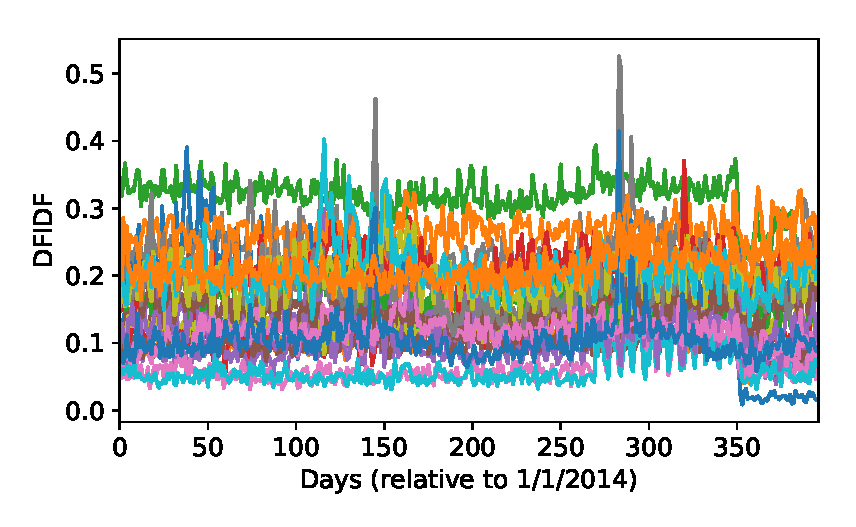
\includegraphics[width=\linewidth]{12_words}  % noisy keywords
  \caption{Event keyword trajectories}
  \label{fig:noisy-keywords}
\end{subfigure}%
\begin{subfigure}{.5\textwidth}
  \centering
  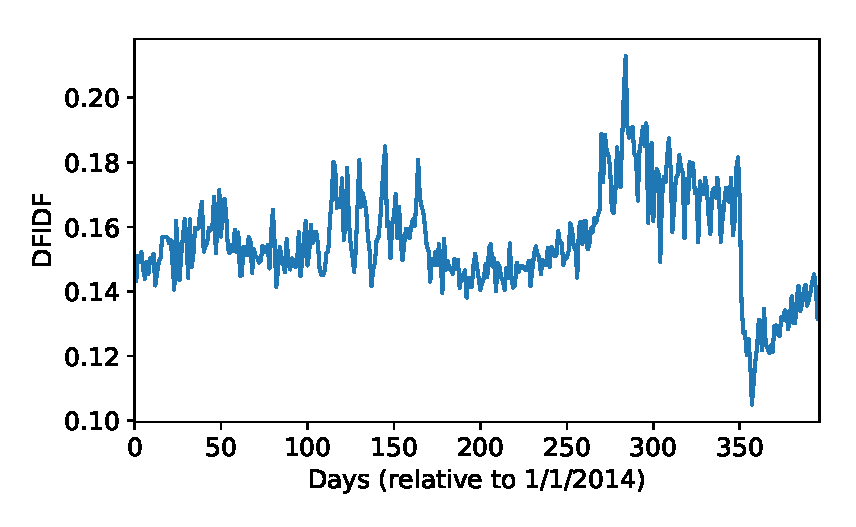
\includegraphics[width=\linewidth]{12_trajectory}  % noisy trajectory
  \caption{Trajectory of the same event}
  \label{fig:noisy-trajectory}
\end{subfigure}
\caption{(a) Event with noisy keywords and trajectory. The keywords are \textit{top, autor (author), podnik (business), test, fotogalerie (photogallery), reklama (advertisement), výsledek (result), komentář (commentary), zpravodajství (reporting), hra (game), informace (information), novinka (hot news), akce (action), návrh (proposition), Martin, klíčový (key, adj.), vedení (leadership), projekt (project), program, účast (participation), ČTK (Czech News Agency)}. (b) Trajectory of the same event constructed from the keywords.}
\end{figure} \label{fig:noisy-event}


\hspace{\fill}

\begin{minipage}{\linewidth}
\centering
\begin{tabular}{ l c }\toprule[1.5pt]
\bf Method 	 & \bf Noisiness \\ \midrule
\bf Original &  50.94\% \\
\bf Greedy   &  19.57\% \\
\bf Cluster &  \bf 19.48\% \\ \bottomrule[1.25pt]
\end {tabular}\par
\captionof{table}{Noisiness comparison} \label{tab:title} 
\end{minipage}

\hspace{\fill}

Here, the cluster-based method performed the best, as the clustering algorithm chosen (DBSCAN) is capable of automatic filtering of noisy samples. With the distance function measuring both trajectory and keyword similarity, it filters out words unrelated to any event.

Surprisingly, the greedy method performed only slighly worse than the cluster-based method. Although the greedy method reached considerable redundancy, manual check revealed that the events mostly consist of important keywords, and most of the trajectories contain distinguiushable bursts.

Poor performance of the original method is partially caused by its large redundancy. Even if a number of words with noisy trajectories appears in similar documents, the method would not group them together to a single event, but split into several noisy events. All of these noisy events then negatively contribute to the noisiness score.

\section{Purity} \label{sec:purity}

All previous evaluations concerned the events on the keyword level. The purity measure will evaluate the event document sets in terms of topical consistency. This is a metric used by \cite{document-purity} and the definition can be found in \cite{information-retrieval}.

The evaluation is an application of the standard measure of cluster purity in the sense that we measure the consistency of class labelling within each cluster. Each event is interpreted as a cluster of documents. Clearly, a high quality event should contain documents concerning similar topics. The problem is that our documents do not have any notion of class labels denoting their topics, which we will have to supplement.

Similarly to \cite{document-purity}, we first assembled a list of 50 words from 1000 most often occurring Nouns and Verbs in document headlines. The words are \textit{Ukrajina (Ukraine), Rusko (Russia), policie (police), soud (court), Zeman, EU, Sparta, festival, Babiš, Putin, Google, ekonomika (economics), letadlo (airplane), východ (east), politika (politics), zabít (to kill), poslanec (deputy), armáda (army), Kyjev (Kiev), Škoda, hokejista (hockey player), fotbalista (football player), doprava (traffic), vražda (murder), Vánoce (Christmas), Francie (France), sport, NATO, Moskva (Moscow), ropa (petroleum), turnaj (tournament), Obama, referendum, ebola, parlament (parliament), koalice (coalition), Paříž (Paris), automobil, mistrovství (championship), elektrárna (power plant), Sýrie (Syria), islamista (islamist), Brusel (Brussels), olympiáda (olympics), sníh (snow), průmysl (industry), revoluce (revolution), výbuch (explosion), finance, terorista (terrorist)}. All documents that contained any of these words in their headline were tagged with the corresponding class label.

Then, for each event, we computed the number of documents tagged by the most frequent label in the event. These values are then summed over all events and divided by the total number of tagged documents from all events.

Mathematically, this is formulated as

\begin{equation}
	\text{Purity} = \frac{1}{\left| \text{Tagged} \right|} \sum_{e \in \text{Events}}{\max_{t \in \text{Tags}} {\left| \{ d \in \doc{e} \mid d.\mathit{tag} = t \} \right|} },
\end{equation}

where $\text{Tagged} = \bigcup_{e \in \text{Events}}{\{ d \in \doc{e} \mid d.\mathit{tag} \text{ is defined} \}}$ and $\text{Tags}$ is a set containing the 50 manually selected words. The results are shown in \autoref{tab:purity}.

\hspace{\fill}

\begin{minipage}{\linewidth}
\centering
\begin{tabular}{ l c }\toprule[1.5pt]
\bf Method 	 & \bf Purity \\ \midrule
\bf Original &  30.53\% \\
\bf Greedy   &  44.42\% \\
\bf Cluster &  \bf 61.08\% \\ \bottomrule[1.25pt]
\end {tabular}\par
\captionof{table}{Purity comparison} \label{tab:purity} 
\end{minipage}

\hspace{\fill}

Poor performance of the original method can be explained by the events consisting mostly of 2 keywords. Such short query for the document collection does not distinguish the documents very well, often retrieving unrelated texts.

The other two methods yield events generally containing more keywords, so the queries are more specific. This allowed the Word Mover's Distance to retrieve more related documents.

\section{Computation time}

Finally, we evaluate the computation time. We measure the execution time of the individual detection steps, so it is clear which parts are the bottlenecks. All experiments were performed on a laptop computer with a 64bit operating system, quad-core processor and 8GB RAM.

In the greedy and cluster-based methods, we did not retrieve documents for periodic events with a period of 7 days or lower. The reason is that such short periods will essentialy cover the entire stream with short bursts and the Word Mover's Distance, computationally expensive on its own, will need to be computed to almost all documents. This might take a day's worth of time, and the short period events mostly concern unineresting events such as sport matches, weather forecasts, etc.

In addition, the summaries were extracted only using 50 most relevant documents, so that the overall process would not take too long.

\hspace{\fill}

\begin{minipage}{\linewidth}
\centering
\begin{tabular}{ r c c c }\toprule[1.5pt]
\bf Unit & \bf Original & \bf Greedy & \bf Clusters \\ \midrule
Word2Vec embedding & --- & \multicolumn{2}{c}{3h 50min} \\
Bag of words model construction & \multicolumn{3}{c}{37min} \\
Word trajectories \& spectral analysis & \multicolumn{3}{c}{8s} \\
Event detection & 2min 12s & 38s & 4min 50s \\
Document retrieval & 7min 30s & 6h & 7h 40min \\
Event annotation & 3h 13min & 8min 20s & 7min 30s \\ \midrule
\bf Total & 4h & 10h 36min & 12h 20min\\ \bottomrule[1.25pt]

\end{tabular}\par
\captionof{table}{Computation time comparison} \label{tab:title}
\end{minipage}

\hspace{\fill}

The original method's document retrieval took considerably less time than the other two methods. The reason is that the original method does not use the Word Mover's Distance as a similarity measure. Due to word semantic similarity being measured only in terms of their document overlap, there is always at least one document containing all the event keywords. It is sufficient to take the documents containing either of the event keywords and intersect these sets, which is much faster than calculating the distance.

This is also the reason why the event annotation took longer in the original method. Having also retrieved documents for events with short period (7 days and less), it is necessary to summarize each period independently. When we summarized only aperiodic events and those with period higher than 7 days, summarization took 1h 12min.



\chapter{Conclusion and future work}
\label{chap:conclusion}
We examined how event detection methods depending on keyword representation could be improved by considering word embedding models, namely the Word2Vec model \citep{word2vec}. We tried to augment an existing method by \cite{event-detection} to use a Word2Vec-based similarity function to match semantically related words together. This did not bring significant improvement -- although the detected events were richer and less redundant, a notable amount of noise appeared. This made the events hard to assign to their real world counterparts, as most of their keywords did not contribute to any underlying topic.

Then, we explored a different approach, where we interpreted the keyword-based event detection as a literal clustering task. We defined a custom distance function also utilizing the Word2Vec model as a semantic measure. We then applied a clustering algorithm equipped with this distance function to words previously selected as eventful. Our evaluation suggests that this method was more successful than both the original method and its Word2Vec modification. The resulting events were composed mostly of representative words and reached lesser redundancy and noisiness than the previous methods.

The disadvantage of both our methods is the necessity to train the Word2Vec model, which is time consuming. However, it can be trained once and than reused for subsequent detections, as long as the document vocabulary remains similar.

We also examined how the Word2Vec model could be used to retrieve documents concerning the detected events. We applied the Word Mover's Distance \citep{wmd} to documents within each event's bursty period as a measure of their relevance to that particular event's keyword set. We then selected the most relevant documents as the event's document representation. Although the documents were of high quality and represented the events well, the process took an unbearable amount of time. In the original method, the retrieval process was more straightforward and much more efficient.

Finally, we applied multi-document summarization techniques to the documents to obtain a short summary describing each event. This, along with the event's occurrence dates and document sets, are the outputs of our method presented to the user. The summaries serve the purpose of giving a quick reference of the event's topic, based on which the user may decide to examine the event further and go through the retrieved documents.

In future work, it would be beneficial to use a more efficient way of computing the documents relevant to each event. Traditional information retrieval techniques, such as Latent Semantic Indexing \citep{lsi} could be used here, perhaps with some domain specific knowledge of the underlying events, such as their bursty periods.

Also, we would like to examine how an event could be represented directly as a set of documents, rather than words. Although there are attempts to do so \citep{document-bursty-representation}, they require to fine-tune a number of parameters, and the document representation is again constructed using word trajectories. The Doc2Vec model \citep{doc2vec}, a generalization of Word2Vec able to embed whole documents in a vector space, could be used to obtain the semantic representation.

Instead of computing a cutoff value to clean a word or an event trajectory, as we did in \autoref{chap:event-detection}, further signal processing techniques could be applied on the trajectories to separate the dominant bursts from the underlying noise. The result would be a somewhat cleaner trajectory devoid of any milder bursts of no interest. This could lower the noisiness, since words would be matched together based on only the dominant activity, not any underlying influence, which still eludes the cutoff value method.


% Bibliography
\bibliography{tex/references}


% Appendices
\appendix
\chapter{Real events used for evaluation}
\label{app:real-events}
This is a list of confirmed events which occurred in 2014 that was used to evaluate Precision and Recall.

\begin{tabularx}{\linewidth}{@{}c @{}c X@{}}\toprule[1.5pt]
\bf \# & \bf Date & \bf Headline \\ \midrule
1 & June 2 & Španělský král Juan Carlos I. abdikoval a za svého nástupce určil svého syna Filipa. \\ \midrule
2 & June 4-5 & Konal se 40. summit G8 v Bruselu. \\ \midrule
3 & June 7 & Petro Porošenko složil prezidentskou přísahu a stal se prezidentem Ukrajiny. \\ \midrule
4 & June 8 & Abd al-Fattáh as-Sísí složil prezidentskou přísahu a stal se prezidentem Egypta. \\ \midrule
5 & June 10 & V izraelských prezidentských volbách byl zvolen Re'uven Rivlin. \\ \midrule
6 & June 12 & V Brazílii začalo 20. mistrovství světa ve fotbale. \\ \midrule
7 & June 15 & Andrej Kiska složil prezidentskou přísahu a stal se prezidentem Slovenska. \\ \midrule
8 & June 18 & Vůdci vojenského převratu v Turecku z roku 1980 Kenan Evren a Tahsin Şahinkaya byli odsouzeni na doživotí. \\ \midrule
9 & June 19 & Filip, asturský kníže složil přísahu a stal se králem Španělska jako Filip VI. Španělský \\ \midrule
10 & July 1 & Itálie se ujala předsednictví EU. \\ \midrule
11 & July 8 & Armáda České republiky utrpěla největší ztrátu v novodobých dějinách, kdy při sebevražedném útoku poblíž letecké základny Bagram zemřeli čtyři čeští vojáci, spolu s dalšími 12 tamními oběťmi. Pátý český voják byl těžce raněn a 14. července zemřel. \\ \midrule
12 & July 13 & Mistry světa ve fotbale se stala německá fotbalová reprezentace. \\ \midrule
13 & July 15 & Novým předsedou Evropské komise se stal lucemburský politik a bývalý premiér Jean-Claude Juncker. \\ \midrule
14 & July 17 & V oblasti bojů na východní Ukrajině se zřítil Boeing 777 malajsijských aerolinií. Zemřelo všech 295 osob na palubě. \\ \midrule
15 & July 21 & Vláda Bohuslava Sobotky vybrala nového eurokomisaře. Stane se jím ministryně pro místní rozvoj Věra Jourová, která ve výběru porazila Pavla Mertlíka. \\ \midrule
16 & August 10 & V historicky první přímé prezidentské volbě v Turecku byl zvolen premiér Recep Tayyip Erdoğan. \\ \midrule
17 & August 16-28 & Letní olympijské hry mládeže 2014 v čínském Nankingu. \\ \midrule
18 & August 19 & Americký novinář James Foley byl popraven v syrské poušti neznámým islámským radikálem, jeho smrt vyvolala v západním světe vlnu pobouření. \\ \midrule
19 & August 24 & Meziplanetární sonda New Horizons prolétla blízko L5 soustavy Slunce–Neptun. \\ \midrule
20 & August 25 & Ve sporu o amnestii Václava Klause soud schválil smír, podle něhož se bývalý hradní právník Pavel Hasenkopf na vyhlášeném znění amnestie nepodílel. \\ \midrule
21 & August 28 & Recep Tayyip Erdoğan složil prezidentskou přísahu a stal se prezidentem Turecka. \\ \midrule
22 & August 30 & Polský premiér Donald Tusk byl na summitu Evropské unie zvolen předsedou Evropské rady. \\ \midrule
23 & September 1 & Pavel Hasenkopf podal na Vratislava Mynáře trestní oznámení pro pomluvu ohledně Mynářova výroku, že Hasenkopf je jedním z autorů amnestie Václava Klause. \\ \midrule
24 & September 2 & Další americký novinář Steven Sotloff byl popraven v syrské poušti neznámým islámským radikálem, stejně jako James Foley v srpnu. \\ \midrule
25 & September 4 & Ve Vilémově se zřítil most, na kterém probíhala rekonstrukce. Zemřeli čtyři dělníci, další dva byli zraněni. \\ \midrule
26 & September 6 & Počet nakažených ebolou při celoroční epidemii se přehoupl přes 4 000. \\ \midrule
27 & September 8 & Britský následník trůnu Princ William a jeho manželka Kate oznámili, že čekají druhé dítě. \\ \midrule
28 & September 10 & Kandidátka na českou eurokomisařku Věra Jourová získala portfolio spravedlnosti, spotřebitelské politiky a rovnosti pohlaví. \\ \midrule
29 & September 13 & Islámští radikálové popravili dalšího západního zajatce, tentokrát jím byl britský humanitární pracovník David Haines. \\ \midrule
30 & September 18 & Ve Skotsku proběhlo referendum o nezávislosti na Spojeném království. Pro odtržení od Británie hlasovalo 44,7\% lidí, proti 55,3\% lidí, Skotsko tak zůstane její součástí. \\ \midrule
31 & September 20 & Náčelník Generálního štábu Armády ČR Petr Pavel byl zvolen předsedou vojenského výboru NATO. \\ \midrule
32 & September 24 & Na Pražský hrad se dostal výhružný dopis adresovaný prezidentovi Miloši Zemanovi s bílým práškem. Případ šetří policie. \\ \midrule
33 & October 3 & Prezident Miloš Zeman přijal demisi ministryně pro místní rozvoj Věry Jourové. \\ \midrule
34 & October 3 & Islámští radikálové popravili dalšího západního zajatce, stal se jím opět britský humanitární pracovník Alan Henning. \\ \midrule
35 & October 7 & Evropský parlament schválil nominaci Věry Jourové na post eurokomisařky pro spravedlnost, spotřebitelskou politiku a rovnost pohlaví. \\ \midrule
36 & October 10-11 & Proběhly volby do Senátu Parlamentu České republiky, volby do zastupitelstev obcí a volby do Zastupitelstva hlavního města Prahy. Ve volbách uspěly především vládní strany ČSSD, ANO a KDU-ČSL. \\ \midrule
37 & October 14 & Žena trpící schizofrenii pobodala na obchodní akademii ve Žďáru nad Sázavou tři studenty a zasahujícího policistu. Jeden ze studentů útok nepřežil. \\ \midrule
38 & October 16 & Ve Vrběticích došlo k výbuchu muničního skladu č. 16. Na místě zahynuli dva zaměstnanci skladu, došlo k evakuaci obyvatel přilehlých obcí. \\ \midrule
39 & October 16 & Zanikla europarlamentní frakce Evropa svobody a přímé demokracie, 20. října byla opět obnovena. \\ \midrule
40 & October 17-18 & Proběhlo druhé kolo voleb do Senátu Parlamentu České republiky. Ve volbách uspěly především vládní strany ČSSD, ANO a KDU-ČSL. \\ \midrule
41 & November 9 & V Katalánsku začalo symbolické hlasování o nezávislosti na Španělsku. \\ \midrule
42 & November 12 & Přistál modul Philae jako historicky první lidský stroj na kometě. \\ \midrule
43 & November 15 & Islámští radikálové popravili dalšího západního zajatce, stal se jím americký humanitární pracovník Peter Kassig. \\ \midrule
44 & November 15-16 & Summit G20 v Brisbane. \\ \midrule
45 & December 1 & Ledovková kalamita ochromila hromadnou dopravu v ČR a dodávky elektřiny v mnoha regionech. Tramvajová doprava v Praze dokonce poprvé ve své historii zažila úplné zastavení provozu. Do normálu se dopravní i energetická situace vrátila až 3. prosince. \\ \midrule
46 & December 1 & Druhým předsedou Evropské rady se stal Donald Tusk. \\ \midrule
47 & December 3 & Ve Vrběticích došlo k dalšímu výbuchu muničního skladu č. 12. Opět proběhla evakuace obyvatel přilehlých obcí, oba dva výbuchy jsou vyšetřovány jako úmyslný trestný čin. \\ \midrule
48 & December 16 & Ozbrojenci ze skupiny Tahrík-e Tálibán-e Pákistán spáchali masakr v péšávarské vojenské škole škole. Útok si vyžádal 141 obětí většinu z nich tvořili děti. \\ \midrule
49 & December 28 & Na cestě ze Surabaje do Singapuru se ztratilo letadlo malajsijské společnosti AirAsia se 162 lidmi na palubě. \\

\bottomrule[1.25pt]
\end{tabularx}

\chapter{Annotated events}
\label{app:clusters-events}
Below are several examples of events detected by the three methods. For each method, we provide examples of Well-formed event summaries as well as those of poor quality. The full outputs for all detected events can be found on the DVD. These examples serve purely to illustrate the various events found using the individual methods.

For each event, the first few keywords are shown to save space. Then, for each event burst, we list its date, headline of the most similar document, and the generated summary with a maximum length of 60 words.

\section{Original method}
\subsection*{Well-formed events}
\begin{tabularx}{\linewidth}{p{\linewidth}} \toprule[1.5pt]

\bf 1. let, mha \\ \midrule
\bf Mar 11 - Apr 2, 2014 \\ \midrule
\bf Pátrání po malajském boeingu pokračuje \\
Což měl údajně být i případ jednoho z lidí v malajsijském letu MH 370. Jsou však značně vzdálené od plánované trasy letu MH 370. Neřekl jsem, že to byl let MH 370. Záhada letu MH 370 pokračuje. Záhada letu MH 370 tak pokračuje. Záhada letu MH 370 trvá. \\ \bottomrule[1.25pt]

\bf Jul 18 - Jul 28, 2014 \\ \midrule
\bf Na Ukrajině byl nejspíš sestřelen malajsijský boeing, více než 300 obětí \\
Zpravodajství o tragickém letu MH 17 najdete v listě. Sestřelení letu MH 17 nadále sledujeme online. Redaktor CNN ukazuje dráhu letu MH 17. Byl MH 17 skutečně sestřelen? Na palubě letu MH 17 bylo podle malajsijského ministra dopravy 298 lidí. Sestřelení letu MH 17 by mu tedy takovou cestu mohlo otevřít. \\ \bottomrule[1.25pt]

\bf Aug 14, 2014 - Jan 5, 2015 \\ \midrule
\bf První zpráva o tragédii letu MH 17 na Ukrajině bude v září \\
První zpráva o tragédii letu MH 17 bude v září. Boeing MH 370 také několikrát prudce změnil výšku. Bratr mi zmizel při letu MH 370, dcera zahynula v MH 17, pláče. Ukrajinská armáda prokazatelně BUKy měla a byly v dobu letu MH 17 aktivní. Separatistka se nalíčila řasenkou oběti letu MH 17. \\ \bottomrule[1.25pt]

\end{tabularx}

\par

\begin{tabularx}{\linewidth}{p{\linewidth}} \toprule[1.5pt]
\bf 2. KDU-ČSL, lidovec \\ \midrule
\bf Jan 4 - Feb 22, 2014 \\ \midrule
\bf Koalice Náměstci, třeste se! \\
Vašimi koaličními partnery jsou ANO a KDU-ČSL. Vláda bude mít 17 členů. Již před Vánoci zveřejnili své nominanty lidovci. Kandidáti hnutí ANO a KDU-ČSL na ministry jsou již známi. KDU-ČSL je stranou, která se často ohání tradicí. ANO i KDU-ČSL budou mít po jenom vicepremiérovi. ANO: Lidovci, rozhodněte se! \\ \bottomrule[1.25pt]

\bf May 16 - Jul 27, 2014 \\ \midrule
\bf Eurovolby 2014 s Janem Kellerem (ČSSD) a Pavlem Svobodou (KDU-ČSL) \\
KDU-ČSL zveřejnila program, se kterým jde do voleb. Proti návrhu je opozice i lidovci. Má podporu zelených a lidovců. To je ale podle lidovců málo. Nové slevy na druhé dítě jsou podle lidovců slabé. Pro lidovce je to však málo. Lidovci nepodpoří Babišovy daňové změny. Lidovcům se to ale zdá málo. \\ \bottomrule[1.25pt]

\bf Oct 11 - Oct 31, 2014 \\ \midrule
\bf SedmiDeník Uplynulý týden očima Kateřiny Perknerové \\
KDU-ČSL kandidují v hlavním městě v Trojkoalici. Zvítězila zde jediná volební kandidátka KDU-ČSL. Věří, že lidovci v obou hlasováních posílí. Lidovci kandují ve dvaceti volebních obvodech. Kandidáti KDU-ČSL vítězili ve třech obvodech, ve dvou pak vedou společní kandidáti lidovců a Strany Zelených. Po sečtení poloviny hlasů vede v komunálních volbách KDU-ČSL. \\ \bottomrule[1.25pt]

\end{tabularx}

\par

\subsection*{Poor quality events}
\begin{tabularx}{\linewidth}{p{\linewidth}} \toprule[1.5pt]

\bf 1. bodovat, děkovat \\ \midrule
\bf Oct 19 - Dec 31, 2014 \\ \midrule
\bf Beránek Začali jsme hrozně. Nevěřil jsem vlastním očím \\
Hemingway bar neboduje jen ve světě. Odpověď zní ``Ne děkuji. V anketě bodovalo divadlo všech žánrů. Pardubice naopak počtvrté za sebou nebodovaly. Východočeši nebodovali už počtvrté za sebou. Réway: Za výhru můžeme děkovat Rasťovi. Mají sílu a teď několikrát za sebou bodovali. JESENÍK BODOVAL V SOUTĚŽI ELEKTROOSKAR. \\ \bottomrule[1.25pt]
\end{tabularx}

\par

\begin{tabularx}{\linewidth}{p{\linewidth}} \toprule[1.5pt]
\bf 2. Čína, čínský \\ \midrule
\bf Apr 19 - Jun 11, 2014 \\ \midrule
\bf Po přidružení k EU se Ukrajina stane jen vývozcem pracovní síly...? (Břetislav Olšer) \\
Nad Čínou se stahují mračna. Na vině je dovoz z Číny. Výsledek je tedy čínskou kopii jiné čínské kopie amerického vozu. McLarenu se v Číně nedaří. V Číně začíná mezinárodní autosalon. Prodej aut v Číně dál poroste. V Číně v sobotu začal mezinárodní autosalon. Fiat bude vyrábět modely Jeep v Číně. \\ \bottomrule[1.25pt]

\bf Oct 10 - Dec 23, 2014 \\ \midrule
\bf Nobelovu cenu za literaturu získal francouzský spisovatel Patrick Modiano \\
Ta bude pod čínskou dominancí a řízená z Pekingu. Vháníme Rusko do náruče Číny. Komunismus je i v Číně, proto je špatná. A doplatí na to výrobci. Ti všichni věří v potenciál růstu čínského akciového trhu. Tento problém už ale bude řešit čínská strana. Ta se v Číně odehraje již dnes. \\ \bottomrule[1.25pt]

\end{tabularx}

\par


\section{Embedded-greedy method}
\subsection*{Well-formed events}

\par

\begin{tabularx}{\linewidth}{p{\linewidth}} \toprule[1.5pt]
\bf 1. sankce, konflikt, Putin, Moskva, západ, východ, armáda, vojenský... \\ \midrule
\bf Jul 26 - Sep 15, 2014 \\ \midrule
\bf Moskva a NATO se hádají o ruské vojáky na Ukrajině \\
Demonstranti v Moskvě žádali Putina o vojenský zásah na Ukrajině. Merkelová: NATO posílí na východě svou vojenskou přítomnost. Vladimir Putin dohlíží na vojenské manévry. Putin chce posílit armádu kvůli údajné hrozbě Západu. Putin prověřuje bojeschopnost armády na Dálném východě. NATO pořádá manévry na západě Ukrajiny, Moskva protestuje. \\ \bottomrule[1.25pt]

\end{tabularx}

\par

\begin{tabularx}{\linewidth}{p{\linewidth}} \toprule[1.5pt]
\bf 2. předplatné, vložit, Václav, Havel, číslo, náměstí, pražský, výročí... \\ \midrule
\bf Oct 26 - Dec 15, 2014 \\ \bf Knihovna Václava Havla slaví 25. výročí sametové revoluce \\
Pro mě to nebyla až taková událost. Hodnotí nejsoučasnější události v Evropě. StB navrhovala zabít Václava Havla. Knihovna Václava Havla slaví 25. výročí sametové revoluce. Oslavy sametové revoluce pohlídají v Praze stovky policistů. Kroměříž si na náměstí připomene výročí revoluce i Karla Kryla. Psali jsme: Čas pracuje pro Václava Havla. \\ \bottomrule[1.25pt]
\end{tabularx}

\par

\subsection*{Poor quality events}
\begin{tabularx}{\linewidth}{p{\linewidth}} \toprule[1.5pt]

\bf 1. únor, březen, loňský, vloni \\ \midrule
\bf Feb 1 - Mar 25, 2014 \\ \midrule
\bf V březnu \\
Co se stalo 20. února? Při loňské razii u Nagyové našla policie šperky za miliony. Tak máme pomalu konec února, jemuž je autor těchto řádků zvyklý říkat úmor. Vyšlo nové vydání Solidarity na únor/březen. Podle nejnovějších zpráv (z 1. března) město Brno povolilo výstavbu skladu Amozonu. \\ \bottomrule[1.25pt]
\end{tabularx}

\par
\newpage

\begin{tabularx}{\linewidth}{p{\linewidth}} \toprule[1.5pt]
\bf 2. útok, oběť, zemřít, boj, těžký, dítě, skončit, Německo... \\ \midrule
\bf Apr 2 - Nov 4, 2014 \\ \midrule
\bf Příměří v Gaze vydrželo dvě hodiny, Izrael pokračuje v bojích. Zemřelo 27 Palestinců \\
Bakterie mají hodiny, které je probudí, když skončí útok antibiotiky. Bakterie mají hodiny, jež je probudí, když skončí útok antibiotiky. Posádka druhého vozu skončila s těžkými zraněními v nemocnici. Těžká nehoda autobusu: Řidič zemřel, těhotná žena skončila popálená! V nemocnici skončilo 33 lidí, tři z nich jsou děti. \\ \bottomrule[1.25pt]

\bf Jan 6 - Jan 26, 2015 \\ \midrule
\bf OBRAZEM Francie vzpomíná na oběti útoků \\
Podle informací deníku Le Monde zemřelo 12 lidí. Zemřelo nejméně 12 lidí, z toho dva policisté. Obama se poklonil obětem pařížského útoku. Útočníci byli Francouzi, narození ve Francii. Část z nich v bojích padla, ale asi 180 radikálů se vrátilo do Německa. Boj proti terorismu: Francie se zbláznila. \\ \bottomrule[1.25pt]

\end{tabularx}
\par


\section{Cluster-based method}
\subsection*{Well-formed events}
\begin{tabularx}{\linewidth}{p{\linewidth}} \toprule[1.5pt]
\bf 1. Gaza, Hamas, Izrael, Izraelec, Palestinec, izraelský, palestinský \\ \midrule
\bf Apr 28 - Sep 20, 2014 \\ \midrule
\bf Izrael vs. Hamás 3.0 \\
Palestinský Hamas oznámí příměří s Izraelem. Izraelci zaútočili na deset cílů v palestinském Pásmu Gazy. Izraelské nálety na Gazu zabily devět Palestinců. Izraelské tanky vjely do Gazy. Hamas prý v pásmu Gazy zadržel izraelského vojáka. Podle Izraele padl do rukou palestinského Hamasu. Izraelci při útoku na Gazu zabili tři velitele Hamasu. \\ \bottomrule[1.25pt]

\bf Dec 19 - Dec 21, 2014 \\ \midrule
\bf Izrael v pásmu Gazy zaútočil na Hamas \\
Izrael v pátek odpoledne oznámil, že Palestinci odpálili z Gazy raketu Kásam. GAZA - Izraelská armáda provedla letecký úder v pásmu Gazy, jehož cílem bylo palestinské hnutí Hamas. Autor: ČTK. Gaza - Izraelská armáda provedla letecký úder v pásmu Gazy, jehož cílem bylo palestinské hnutí Hamas. Přesto s Hamásem nic neudělá. \\ \bottomrule[1.25pt]
\end{tabularx}

\par
\newpage

\begin{tabularx}{\linewidth}{p{\linewidth}} \toprule[1.5pt]
\bf 2. Ebola, Guinea, Leone, Libérie, Sierra, ebola, epidemie \\ \midrule
\bf Sep 28 - Oct 29, 2014 \\ \midrule
\bf Epidemie eboly \\
Ebola nejdříve propukla v Guineji. Nejvíce postižené země jsou Sierra Leone, Guinea a Libérie. Libérie je spolu se Sierrou Leone a Guineou nejpostiženější ze západoafrických zemí. Zatím epidemie eboly hlavně postihovala východ Sierra Leone. Libérie patří k zemím nejvíce zasaženým epidemií eboly. WHO: Epidemie eboly v Libérii začala ustupovat. \\ \bottomrule[1.25pt]
\end{tabularx}
\par

\subsection*{Poor quality events}

\begin{tabularx}{\linewidth}{p{\linewidth}} \toprule[1.5pt]
\bf 1. extra, podnik, reklama, siga, zpravodajství \\ \midrule
\bf Oct 10 - Dec 3, 2014 \\ \midrule
\bf Maturus o. p. s. \\
Jaké reklamy na vás působí nejvíce? Reklama na mě nemá téměř žádný vliv. Televize Barrandov v listopadu rozšíří zpravodajství. Některé reklamy jsou hodně odvážné. Jaké se ti líbí reklamy? 4. Jaké se ti líbí reklamy ? 9. Zajímavá jsou zjištění ohledně televizní reklamy. Tyto reklamy se mi líbí. 3. \\ \bottomrule[1.25pt]
\end{tabularx}

\par

\begin{tabularx}{\linewidth}{p{\linewidth}} \toprule[1.5pt]
\bf 2. Rusko, ruský \\ \midrule
\bf Feb 21 - Apr 24, 2014 \\ \midrule
\bf RUSKÝ POSTKOLONIALISMUS - 1. \\
Jaké jsou skutečné možnosti Ruska? Rusko potřebuje investory jako sůl. Na budově zavlál prapor Ruska. Tak to je pro Rusko dárek! Lid žádá návrat do Ruska. Rusko, největší stát světa, se může radovat. Tím se dostala i západní Ukrajina pod ruskou vládu. Rusko nemělo evidentně zájmy ve střední Evropě. \\ \bottomrule[1.25pt]

\bf Jul 28 - Sep 8, 2014 \\ \midrule
\bf Hurá na Rusko \\
Bát bychom se neměli Ruska, ale USA a EU. Rusko se vyhnulo klasickému otroctví. Za Janukoviče byly zájmy Ruska v bezpečí. Upozornil na to ruský server newsru.com. Rusko se obává, že se EU zřekne ruských raket. Válčí Rusko na Ukrajině? Vše na ruské straně proběhlo dobře. \\ \bottomrule[1.25pt]

\bf Nov 30 - Jan 8, 2015 \\ \midrule
\bf Rusko \\
Ne že by na to Rusko nemělo. Reálně není Rusko nikým vojenský ohrožováno. Odvolejme naše sankce proti Rusku! Zhruba v polovině léta se k ní přidal i ruský rubl. Rusko nejen přežije, ale bude mnohem silnější, řekl. Ruská centrální banka zahájila intervence na posílení rublu. Rusko tato nařčení opakovaně odmítlo. \\ \bottomrule[1.25pt]
\end{tabularx}


\par


\end{document}